% Copyright 2004 by Till Tantau <tantau@users.sourceforge.net>.
%
% In principle, this file can be redistributed and/or modified under
% the terms of the GNU Public License, version 2.
%
% However, this file is supposed to be a template to be modified
% for your own needs. For this reason, if you use this file as a
% template and not specifically distribute it as part of a another
% package/program, I grant the extra permission to freely copy and
% modify this file as you see fit and even to delete this copyright
% notice. 

\documentclass{beamer}

% There are many different themes available for Beamer. A comprehensive
% list with examples is given here:
% http://deic.uab.es/~iblanes/beamer_gallery/index_by_theme.html
% You can uncomment the themes below if you would like to use a different

%\usetheme{AnnArbor}
%\usetheme{Antibes}
%\usetheme{Bergen}
%\usetheme{Berkeley}
%\usetheme{Berlin}
%\usetheme{Boadilla}
%\usetheme{boxes}
%\usetheme{CambridgeUS}
%\usetheme{Copenhagen}
%\usetheme{Darmstadt}
%\usetheme{default}
%\usetheme{Frankfurt}
%\usetheme{Goettingen}
%\usetheme{Hannover}
%\usetheme{Ilmenau}
%\usetheme{JuanLesPins}
%\usetheme{Luebeck}
%\usetheme{Madrid}
%\usetheme{Malmoe}
%\usetheme{Marburg}
%\usetheme{Montpellier}
%\usetheme{PaloAlto}
%\usetheme{Pittsburgh}
%\usetheme{Rochester}
%\usetheme{Singapore}
%\usetheme{Szeged}
%\usetheme{Warsaw}
%\usetheme{metropolis}

\title{Lagrangian geographies of the Gulf of Mexico}

% A subtitle is optional and this may be deleted
%\subtitle{Optional Subtitle}

\author{P. Miron\inst{1}, F.J. Beron-Vera\inst{1}, M.J. Olascoaga\inst{1}, P. P\'erez-Brunius\inst{2} and J. Sheinbaum\inst{2}}

\institute % (optional, but mostly needed)
{
  \inst{1}%
  Rosenstiel School of Marine and Atmospheric Science\\
  University of Miami
  \and
  \inst{2}%
  Centro de Investigaci\'on Cient\'ifica y de Educaci\'on Superior de Ensenada, B\
  Ensenada, Baja California, Mexico
}
% - Use the \inst command only if there are several affiliations.
% - Keep it simple, no one is interested in your street address.

\date{LAPCOD, Venezia, 2019}
% - Either use conference name or its abbreviation.
% - Not really informative to the audience, more for people (including
%   yourself) who are reading the slides online

\subject{Theoretical Computer Science}
% This is only inserted into the PDF information catalog. Can be left
% out. 

% Beamer settings
\setbeamertemplate{navigation symbols}{} %remove nav symbols
\setbeamertemplate{bibliography item}{}
\setbeamertemplate{footline}[frame number]

% If you have a file called "university-logo-filename.xxx", where xxx
% is a graphic format that can be processed by latex or pdflatex,
% resp., then you can add a logo as follows:

%\graphicspath{{"2019. mh370/figures/"}}
\graphicspath{{"figures/"}}

% \pgfdeclareimage[height=0.5cm]{university-logo}{university-logo-filename}
% \logo{\pgfuseimage{university-logo}}
\titlegraphic{
\begin{tikzpicture}[overlay, remember picture]
%\node[at=(current page.south west), anchor=south west] {%
% 
\includegraphics[height=.10\textwidth]{carthe.png} 
%};
\node[at=(current page.south west), anchor=south west] {%
 
\includegraphics[height=.18\textwidth]{cigom.jpg} 
};
\node[at=(current page.south east), anchor=south east] {
 
\includegraphics[height=.14\textwidth]{GoMRi.png}
};
\end{tikzpicture}
}

% Delete this, if you do not want the table of contents to pop up at
% the beginning of each subsection:
%\AtBeginSubsection[]
%{
%  \begin{frame}<beamer>{Outline}
%    \tableofcontents[currentsection,currentsubsection]
%  \end{frame}
%}

% bibliography
\usepackage[style=authoryear, sortcites=true, sorting=nyt, giveninits=true, uniquename=init, doi=false, url=false, isbn=false, eprint=false]{biblatex}
\addbibresource{oce.bib}
% remove annoying biblatex bug/warning
\usepackage{silence}
\WarningFilter{biblatex}{Patching footnotes failed}

% some definitions
\usepackage[utf8]{inputenc}
\usepackage[english]{babel}
\usepackage{amssymb}
\usepackage{amsfonts}
\usepackage{amsmath}
\usepackage{bbold}
\usepackage{ragged2e} % justify text in all frame
\apptocmd{\frame}{}{\justifying}{}
\usepackage{etoolbox}
\usepackage{xcolor}
\usepackage{tikz}
\usepackage{subfig}
\usepackage{multicol}
\usepackage{siunitx}
\usepackage{csquotes}
\usepackage{hyperref}
\usepackage{tikz,pgfplots}
\pgfplotsset{compat=1.12}

% Definitions.
\DeclareMathOperator{\area}{area}%
\DeclareMathOperator{\Id}{Id}%
\newcommand{\PF}{\mathcal{P}}
\newcommand{\ia}{\textit{a}}
\newcommand{\ib}{\textit{b}}
\newcommand{\ic}{\textit{c}}
\newcommand{\id}{\textit{d}}
\newcommand{\ie}{\textit{e}}
\newcommand{\gom}{GoM}
\let\vaccent=\v 
\renewcommand{\v}[1]{\ensuremath{\mathbf{#1}}} 
\newcommand{\minus}{\scalebox{0.5}[1.0]{$-$}}
\newcommand{\dif}{\ensuremath{\text{d}}}

\def\pct{\%}
\renewcommand{\d}[1]{\ensuremath{\operatorname{d}\!{#1}}}
\renewcommand{\Pr}{\mathop{\rm prob}\nolimits}
\DeclareMathOperator*{\m}{area}
\DeclareMathOperator*{\argmax}{arg\,max}
\DeclareMathOperator*{\argmin}{arg\,min}

\definecolor{xkcd:purple}{HTML}{7e1e9c}
\definecolor{xkcd:green}{HTML}{15b01a}
\definecolor{xkcd:blue}{HTML}{0343df}
\definecolor{xkcd:pink}{HTML}{ff81c0}
\definecolor{xkcd:brown}{HTML}{653700}
\definecolor{xkcd:red}{HTML}{e50000}
\definecolor{xkcd:lightblue}{HTML}{95d0fc}
\definecolor{xkcd:teal}{HTML}{029386}
\definecolor{xkcd:orange}{HTML}{f97306}
\definecolor{xkcd:lightgreen}{HTML}{96f97b}
\definecolor{xkcd:majenta}{HTML}{c20078}
\definecolor{xkcd:grey}{HTML}{929591}
\definecolor{xkcd:lightpurple}{HTML}{bf77f6}
\definecolor{xkcd:turquoise}{HTML}{06c2ac}
\definecolor{xkcd:tan}{HTML}{d1b26f}
\definecolor{xkcd:olive}{HTML}{6e750e}
\definecolor{xkcd:salmon}{HTML}{ff796c}


% Let's get started
\begin{document}

\frame[plain,noframenumbering]{
\titlepage
}

\iffalse
\begin{frame}{Outline}
  \tableofcontents
  % You might wish to add the option [pausesections]
\end{frame}
\fi

\begin{frame}{Introduction}
kjgjhgjydfhtfggfj
\end{frame}

\begin{frame}

\begin{equation*}
  P_{ij} = \Pr[\xi_{t+T}\in B_j \mid \xi_t \in B_i]
\end{equation*}
which can be estimated as 
\begin{equation*}
  P_{ij} \approx \frac{\mbox{\# points in $B_i$ at $t$ that
  evolve to $B_j$ at $t+T$}}{\mbox{\# points in $B_i$ at $t$}}. 
  \label{eq:P}
\end{equation*}

\begin{figure}[hbt]
\centering
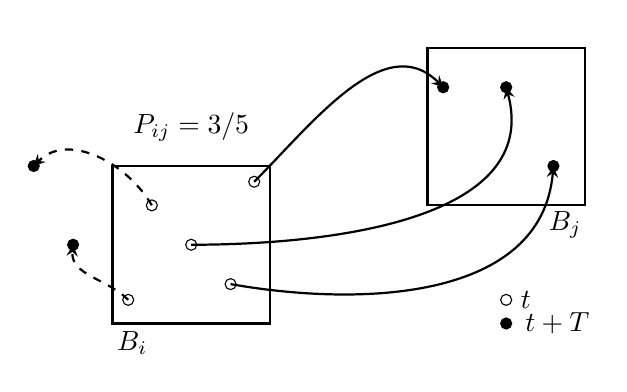
\begin{tikzpicture}
    % two bins
	\draw[thick] (0,0) rectangle (2,2);
	\draw[thick] (4,1.5)   rectangle (4+2,1.5+2);	
	\node at (0.25, -0.25) {$B_i$};
	\node at (5.75, 1.25) {$B_j$};
	\node at (1, 2.5) {$P_{ij} = 3/5$};
	
	% particles def
    \coordinate (A0) at (1.8, 1.8);
    \coordinate (AT) at (4.2, 3);
    \draw (A0) circle (0.07cm);
    \draw[fill=black] (AT) circle (0.07cm);
    
    \coordinate (B0) at (1, 1);
    \coordinate (BT) at (5, 3);
    \draw (B0) circle (0.07cm);
    \draw[fill=black] (BT) circle (0.07cm);
    
    \coordinate (C0) at (1.5, 0.5);
    \coordinate (CT) at (5.6, 2);
    \draw (C0) circle (0.07cm);
    \draw[fill=black] (CT) circle (0.07cm);
    
    \coordinate (D0) at (0.5, 1.5);
    \coordinate (DT) at (-1, 2);
    \draw (D0) circle (0.07cm);
    \draw[fill=black] (DT) circle (0.07cm);
    
    \coordinate (E0) at (0.2, 0.3);
    \coordinate (ET) at (-0.5, 1);
    \draw (E0) circle (0.07cm);
    \draw[fill=black] (ET) circle (0.07cm);
	
	\draw[thick,->,>=stealth] (A0) to [out=45, in=135] (AT);	
	\draw[thick,->,>=stealth] (B0) to [out=0, in=-75] (BT);	
	\draw[thick,->,>=stealth] (C0) to [out=-10, in=-95] (CT);
	\draw[thick,->,>=stealth,dashed] (D0) to [out=120, in=45] (DT);
	\draw[thick,->,>=stealth,dashed] (E0) to [out=135, in=-95] (ET);
	
	\draw (5,0.3) circle (0.07cm);
	\draw[fill=black] (5,0) circle (0.07cm);
	\node at (5.25, 0.3) {$t$};
	\node at (5.65, 0) {$t+T$};
\end{tikzpicture}
\end{figure}
\end{frame}


\frame{\frametitle{Introduction}
RAFOS experiment sponsored by the Bureau of Ocean Energy Management (July 2011 - May 2015)\footnote{Publicly available data sets compiled by WOCE Subsurface Float Data Assembly Center (WFDAC).}:
\begin{itemize}
\item 4-year-long program (floats $\sim 2$-y mission)
\item 121 floats at 1500\,m
\item 6 profiling floats with RAFOS technology at 1500\,m
\item 31 floats at 2500\,m
\end{itemize}

\begin{figure}
    \centering
    %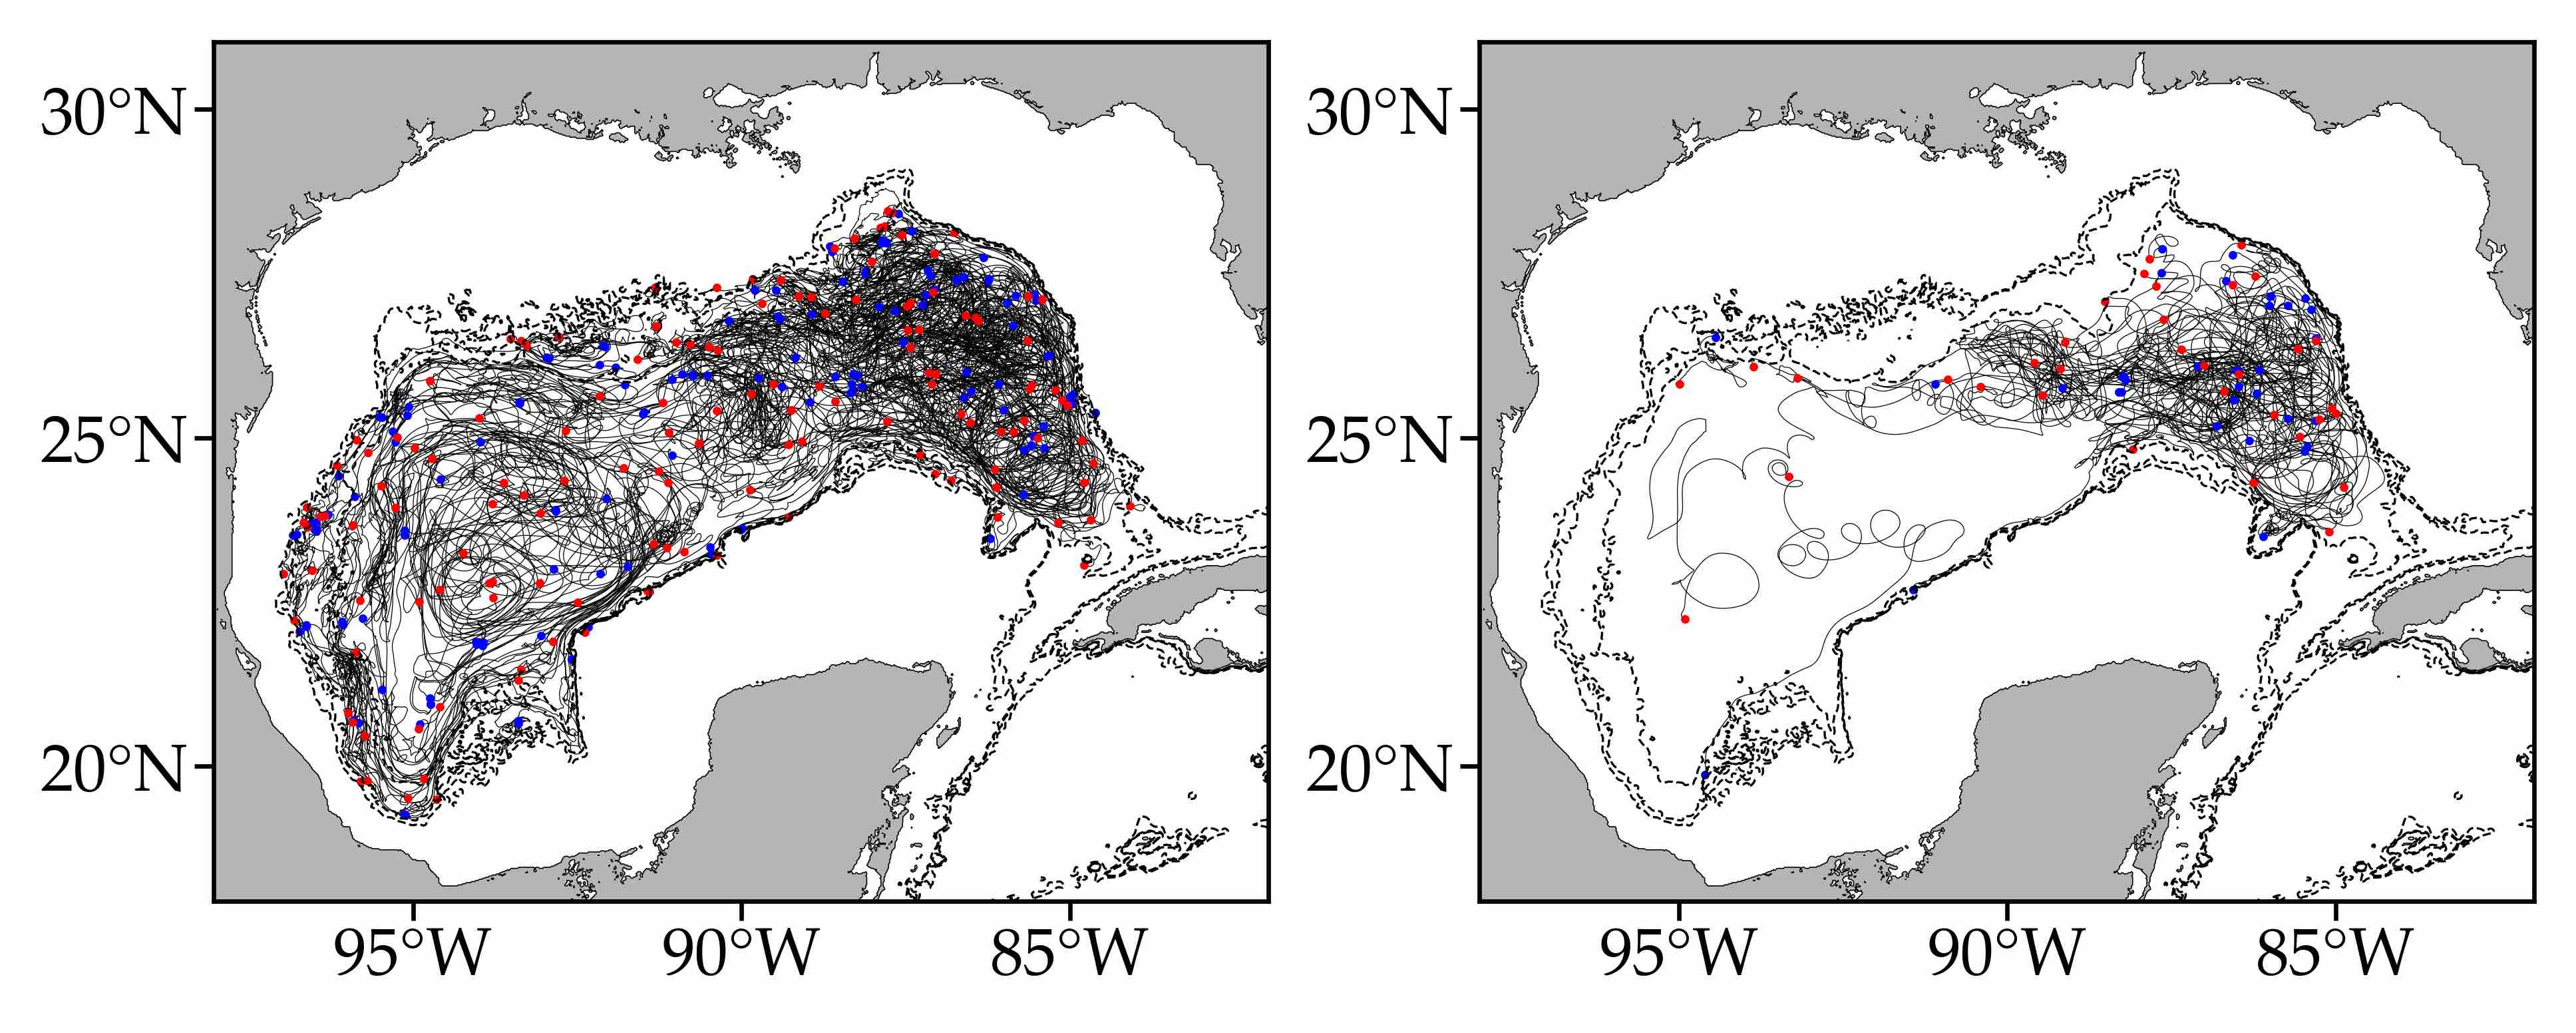
\includegraphics[width=\textwidth]{geogomdeep-fig01}
\end{figure}

}

\section{Objectives}

\frame{\frametitle{Objectives}
Using floats data (trajectories) in the abyssal Gulf of Mexico (\gom):
\begin{itemize}
    \item subdivide the deep \gom\ into regions with similar dynamics;
    \item identify almost invariant regions and their respective timescale;
    \item assess connectivity.
\end{itemize}
}

frame{\frametitle{Theory: how to construct the transition matrix}  

By partitioning the domain $X$ into a grid of $N$ regular connected boxes $\{B_1,\dotsc,B_N\}$ and with large number of initial conditions we can estimate the entries:
\begin{equation}
   \mathcal{P} \approx P_{ij} = \frac{\# x \text{ in }B_i\text{ at any time } t \text{ and in }B_j \text{ at  } t+T}{\#x\text{ in }B_i \text{ at any time }t},
  \label{eq:Pnum}
\end{equation}
which are transitional probabilities of moving from $B_i$ to $B_j$. It defines a \textbf{Markov Chain} (with bins $\equiv$ states) of the dynamics.
\newline\newline
Timescale T is fix at 7-d which is larger then the decorrelation scale of 5-d and enough to allow interbins connection.
}


\frame{\frametitle{Application of the transition matrix}
One can push forward discrete representations of $f(x)$:
\begin{equation}
    \mathbf f = (f_1,\cdots,f_N),
\end{equation}
under left-multiplication by $P$:
\begin{align}
    f^{(1)} &= f\,P \nonumber\\
    f^{(2)} &= f^{(1)}\,P = f\,P^2 \nonumber\\
    f^{(k)} &= f\,P^k
\end{align}
}

\frame{\frametitle{Eigenvectors analysis}

It is also of interest to identify when a distribution $\mathbf f$ is almost invariant:
\begin{equation}
    \mathbf f \approx \mathbf f\,P
\end{equation}

This is available from the \emph{eigenspectrum} inspection of $P$ \parencite{Froyland-etal-12}.
\newline\newline
If in the matrix $P$:
\begin{itemize}
    \item all states \emph{communicate};
    \item no state occurs \emph{periodically}.
\end{itemize}
$P$ has one $\lambda = 1$ a limiting distribution $\mathbf{p} = \mathbf{p} P$.
\newline\newline
Note: $\mathbf{p}$ is a left eigenvector of $P$ (row-stochastic matrix) with eigenvalue $\lambda = 1$.
\begin{align*}
    \mathbf{p} \lambda &= \mathbf{p} P\\
    \mathbb{1} \lambda &= P\mathbb{1}
\end{align*}
}

\frame{\frametitle{Attractors and basin off attractions}

Motivates the idea that regions where trajectories converge and their basins of attraction are encoded in the eigenvectors of the transition matrix $P$ with eigenvalues ($\lambda \approx 1$) \parencite{Froyland-etal-14}.

\begin{itemize}
    \item \textbf{right eigenvector} of $P$ is the basin of attraction (\textbf{constrains connectivity!})
    \item \textbf{left eigenvector}  of $P$ is the attractor or almost-invariant region
\end{itemize}
}

\frame{\frametitle{Example with a simple 5 states problem}

\begin{figure}[!ht]
  \centering
  %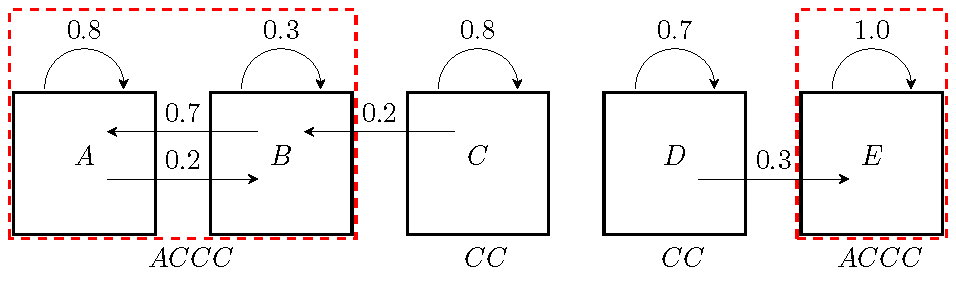
\includegraphics[width=0.9\textwidth]{fig01}
\end{figure}

\only<1>{
\begin{equation*}
\PF = 
  \begin{tabular}{c|ccccc}
    & A & B & C & D & E\\\hline
  A & 0.8 & 0.2 & 0 & 0 & 0\\
  B & 0.7 & 0.3 & 0 & 0 & 0\\
  C & 0 & 0.2 & 0.8 & 0 & 0\\
  D & 0 & 0 & 0 & 0.7 & 0.3\\
  E & 0 & 0 & 0 & 0 & 1.0
  \end{tabular}
  \label{eq:ex_pf}
\end{equation*}
}

\only<2->{
\begin{equation*}
  L_1^T = 
  \begin{pmatrix}
  0.83\\
  0.55\\
  0\\
  0\\
  0\\
  \end{pmatrix}\quad
  R_1 = 
  \begin{pmatrix}
  1\\
  1\\
  1\\
  0\\
  0\\
  \end{pmatrix}\quad
  L_2^T = 
  \begin{pmatrix}
  0\\
  0\\
  0\\
  0\\
  1\\
  \end{pmatrix}\quad
  R_2 = 
  \begin{pmatrix}
  0\\
  0\\
  0\\
  1\\
  1\\
  \end{pmatrix}
\end{equation*}

\begin{multicols}{2}
\begin{itemize}
    \item $L_1$: $A, B$ are attractors
    \item $L_2$: $E$ is another attractor
    \item $R_1$: $A, B, C$ basin of attr.
    \item $R_2$: $D, E$ basin of attr.
\end{itemize}
\end{multicols}
}
}

\frame{\frametitle{Algorithm}

\begin{enumerate}
  \item Split the domain (\gom) into square boxes
  \item For each trajectory segment:
  \begin{itemize}
    \item find bins $i$ where $x_0$ is located and store the segment $ID$ in the vector $B_i$
    \item identify bins $j$ where $x_f$ is located and store the segment $ID$ in the vector $B_j$
  \end{itemize}  
  \item Calculate the transition matrix $\PF_{ij}$ using vectors $B_i$ and $B_j$
  \item Calculate eigenvalues and eigenvectors of $\PF$
\end{enumerate}

}

\section{Results}
\frame{\frametitle{Eigenvectors}

\only<1>{
Eigenvectors associated with $\lambda_1=1$ and $\lambda_2=0.9953$.
\begin{figure}
  %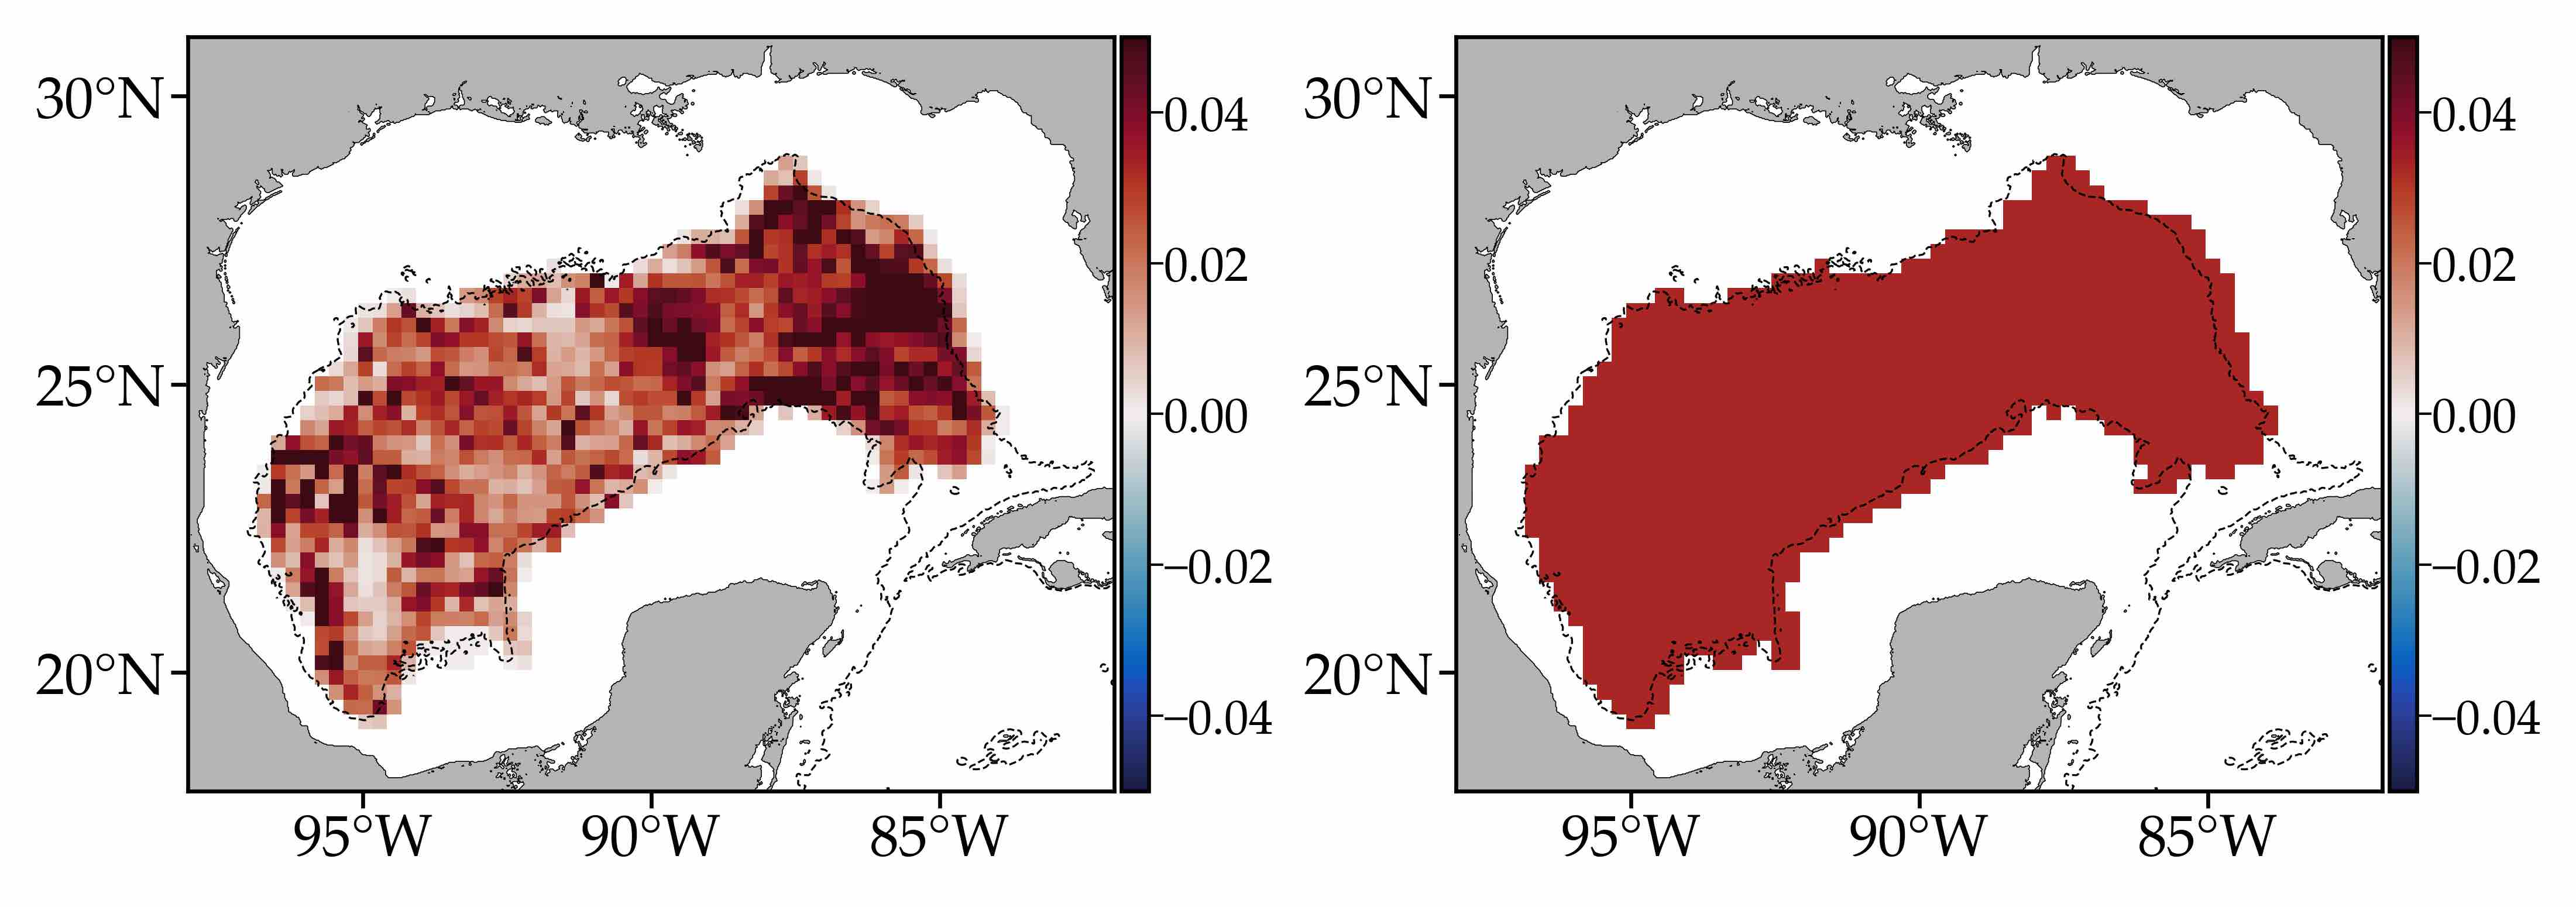
\includegraphics[width=\textwidth]{geogomdeep-fig07.jpg}
\end{figure}
\begin{figure}
  %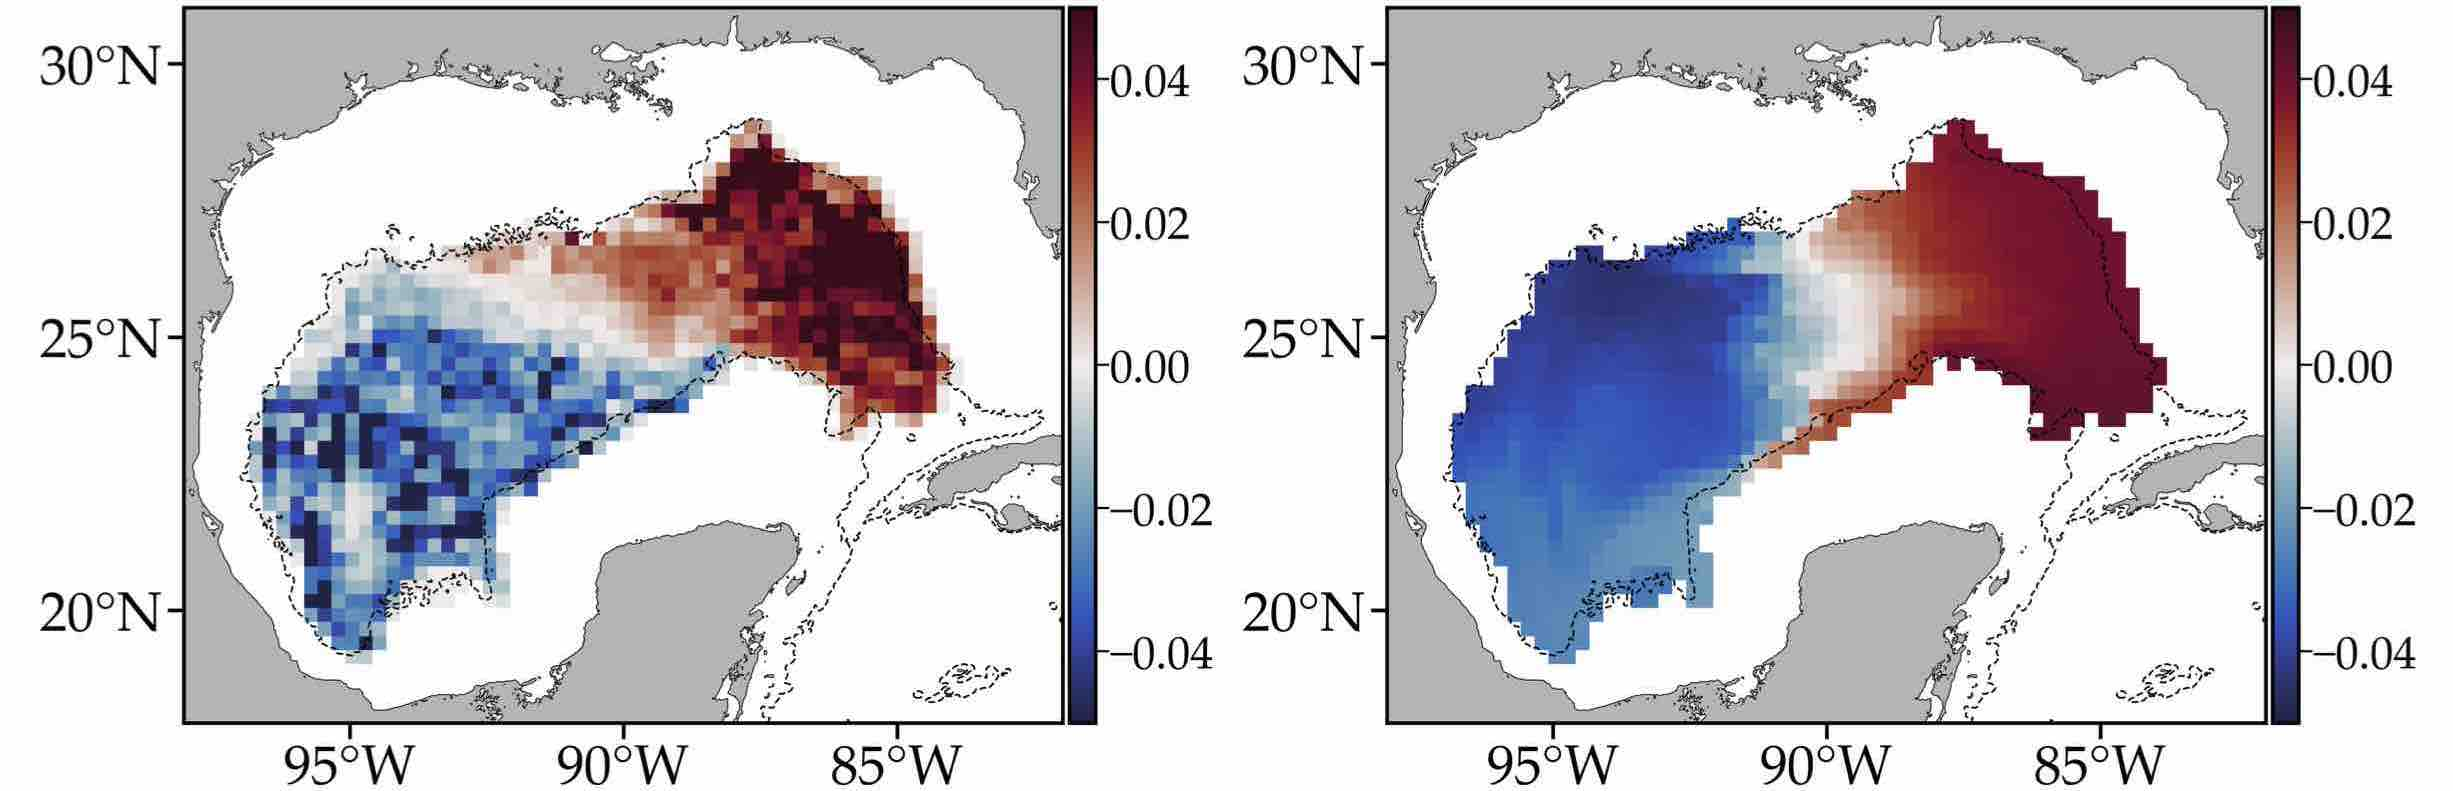
\includegraphics[width=\textwidth]{geogomdeep-fig08a.jpg}
\end{figure}
}

\only<2>{
Eigenvectors associated with $\lambda_3=0.9832$ and $\lambda_5=0.9712$.
\begin{figure}
  %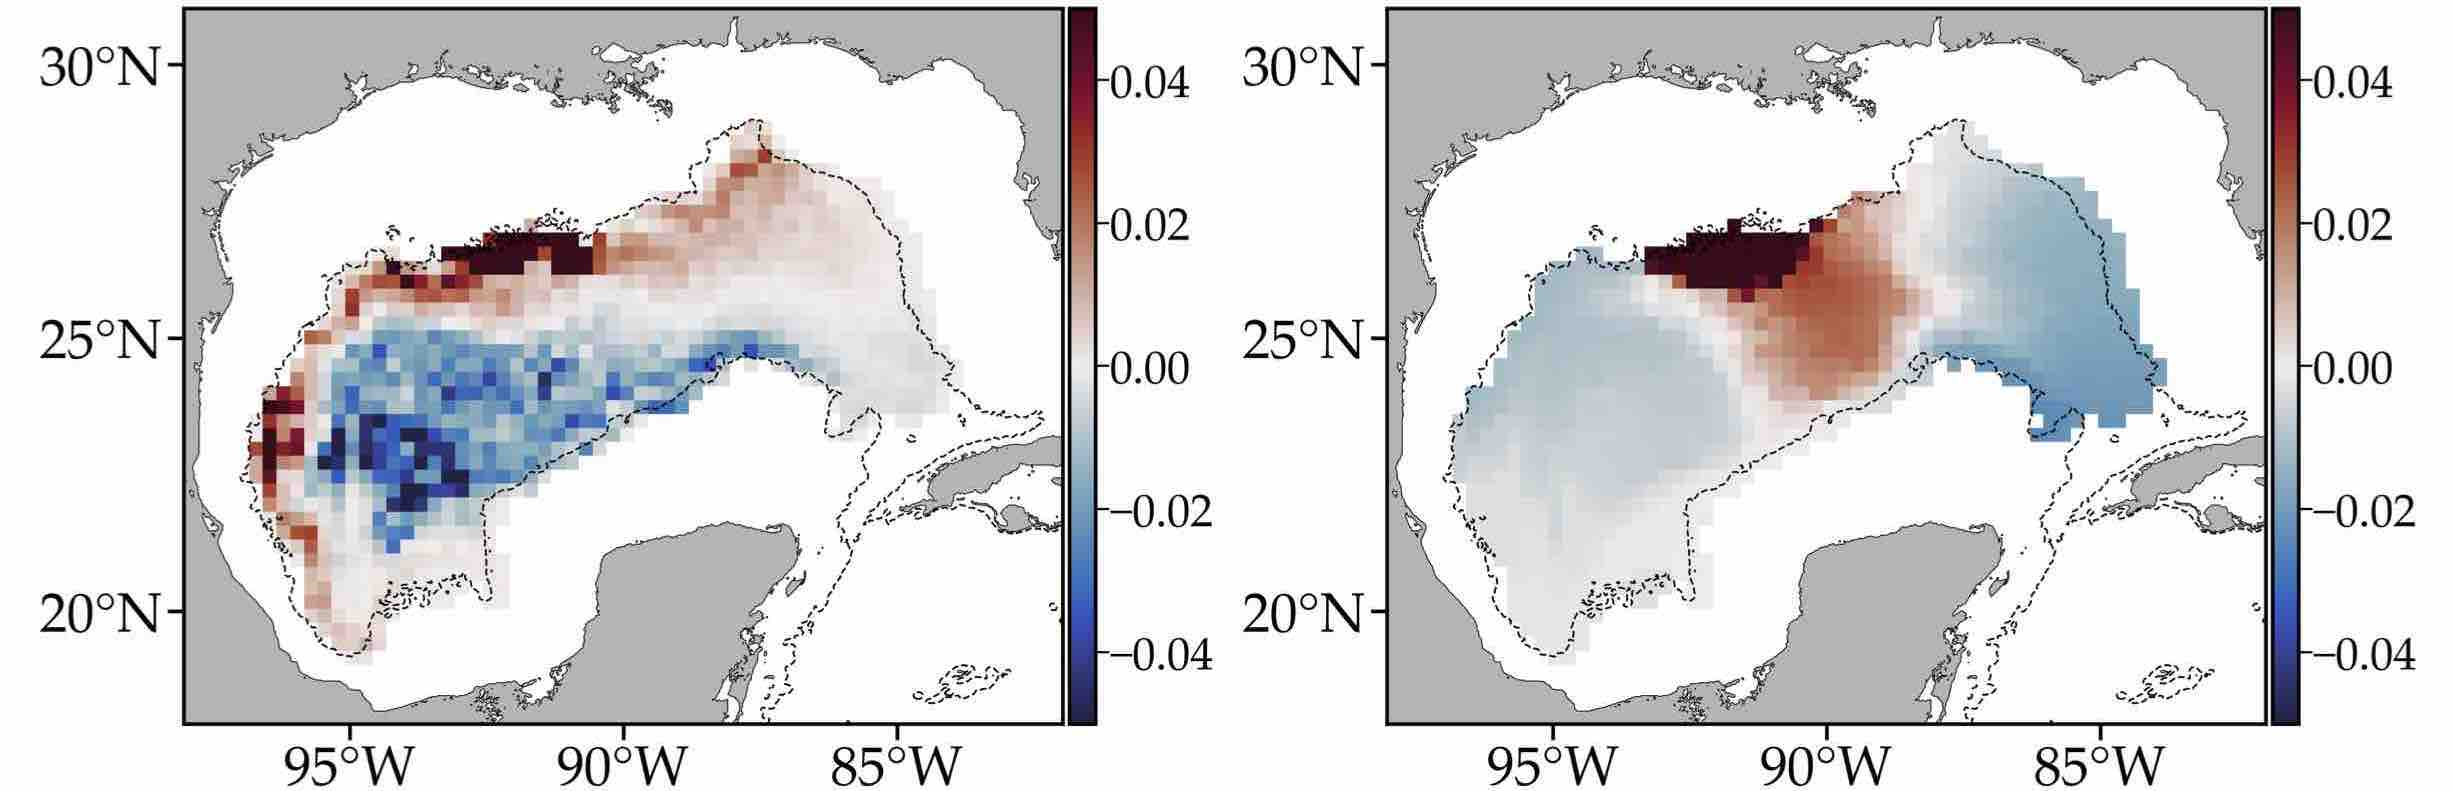
\includegraphics[width=\textwidth]{geogomdeep-fig08b.jpg}
\end{figure}
\begin{figure}
  %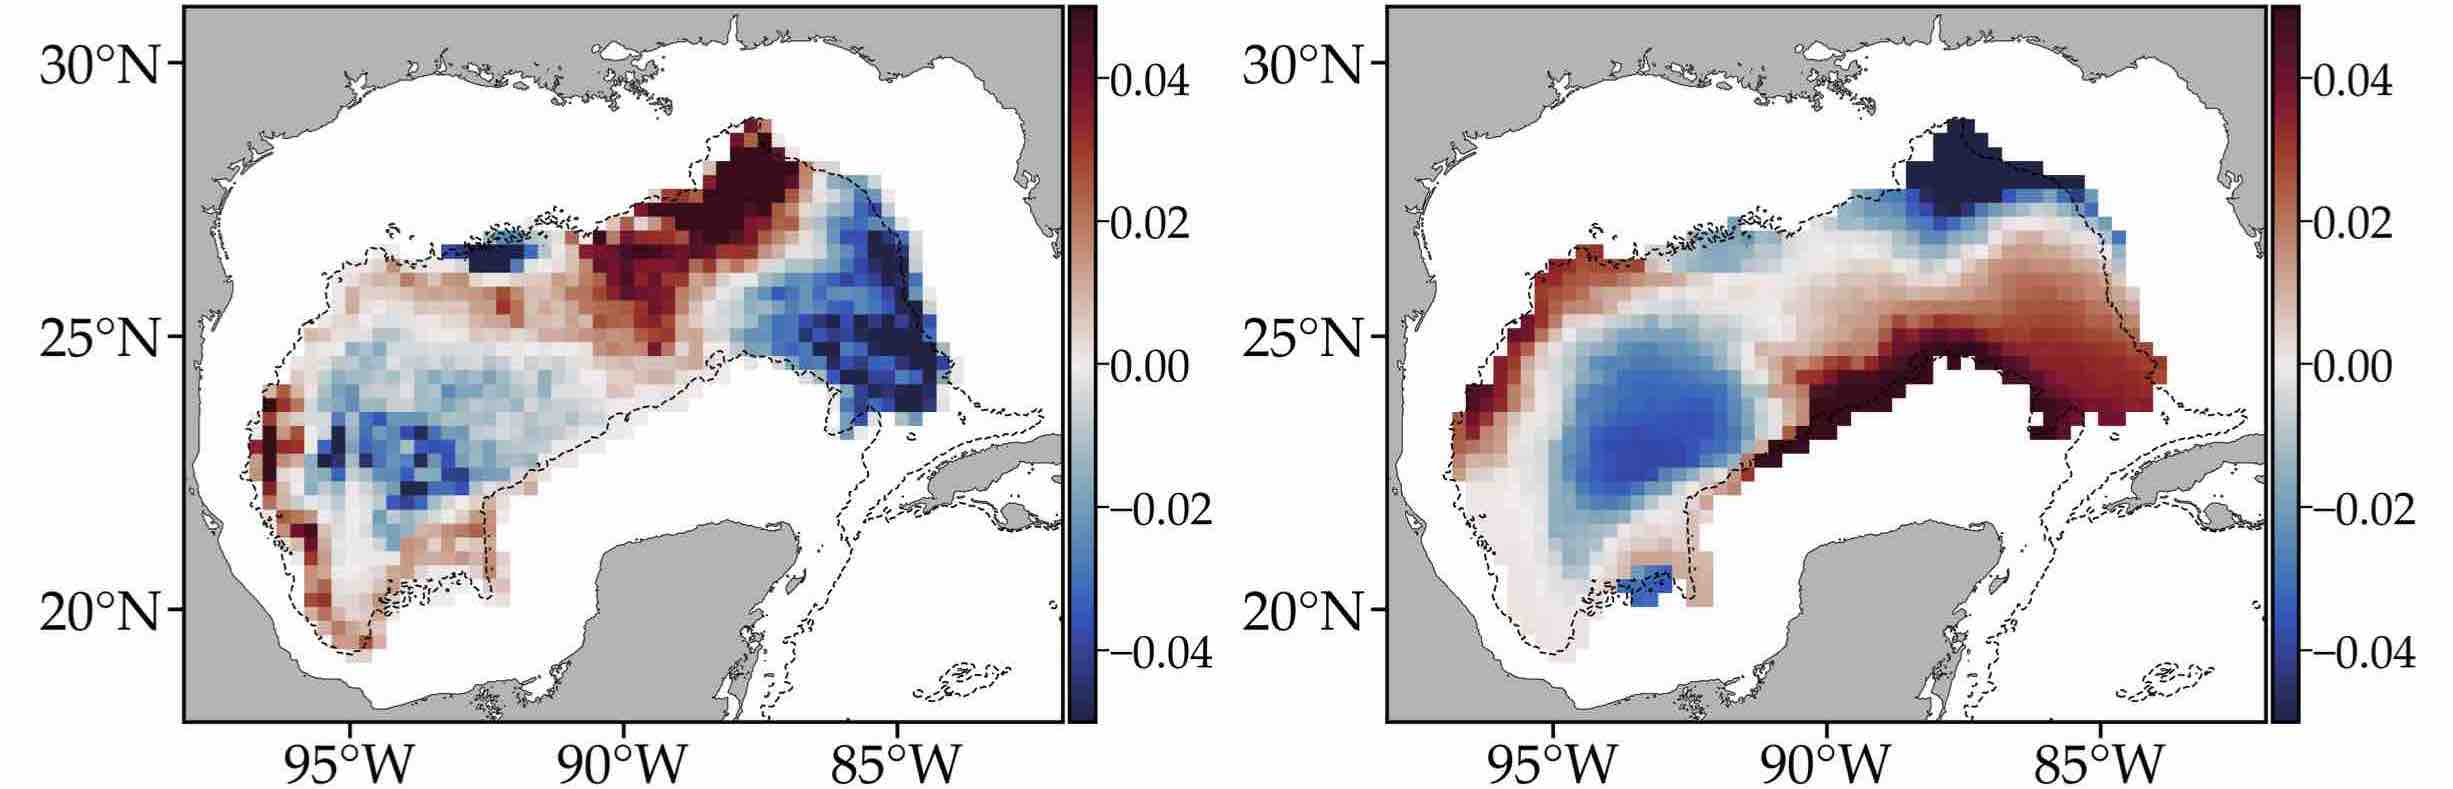
\includegraphics[width=\textwidth]{geogomdeep-fig08c.jpg}
\end{figure}
}
}

\frame{\frametitle{Lagrangian geography of the deep Gulf of Mexico}

Combination of the basins of attraction from the top right eigenvectors (by thresholding).
\begin{figure}
  %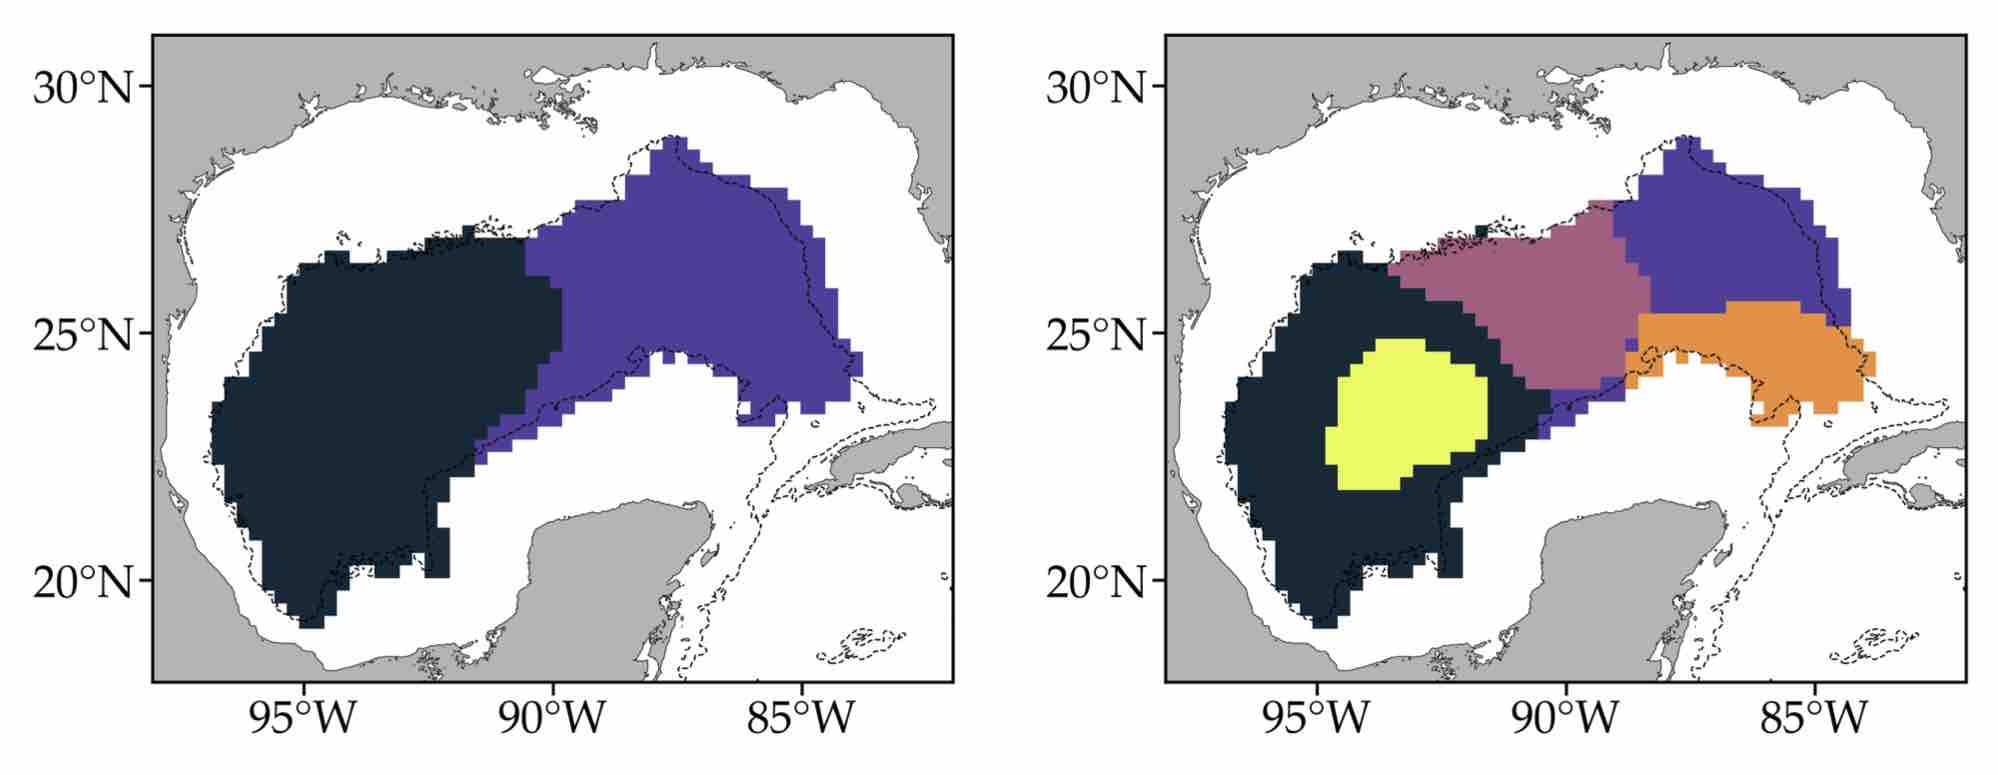
\includegraphics[width=0.9\textwidth]{geogomdeep-fig09.jpg}
\end{figure}

\begin{figure}
  %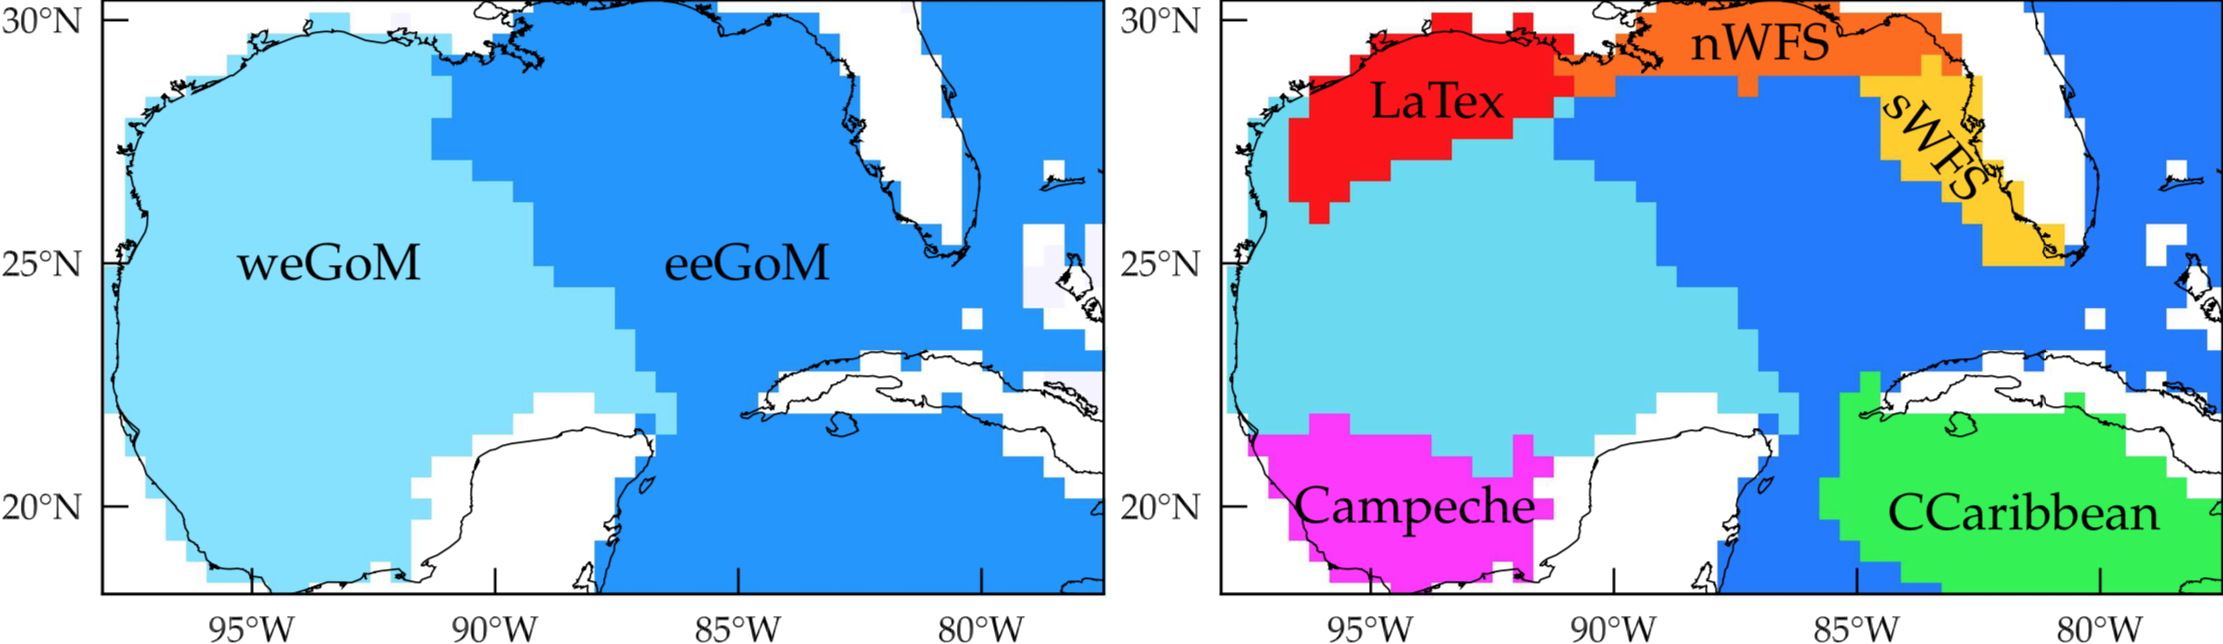
\includegraphics[width=0.9\textwidth]{geosurf.png}
\end{figure}
}

\frame{
\begin{figure}
  \only<1>{
  \frametitle{Connectivity matrix (1 week)}
  %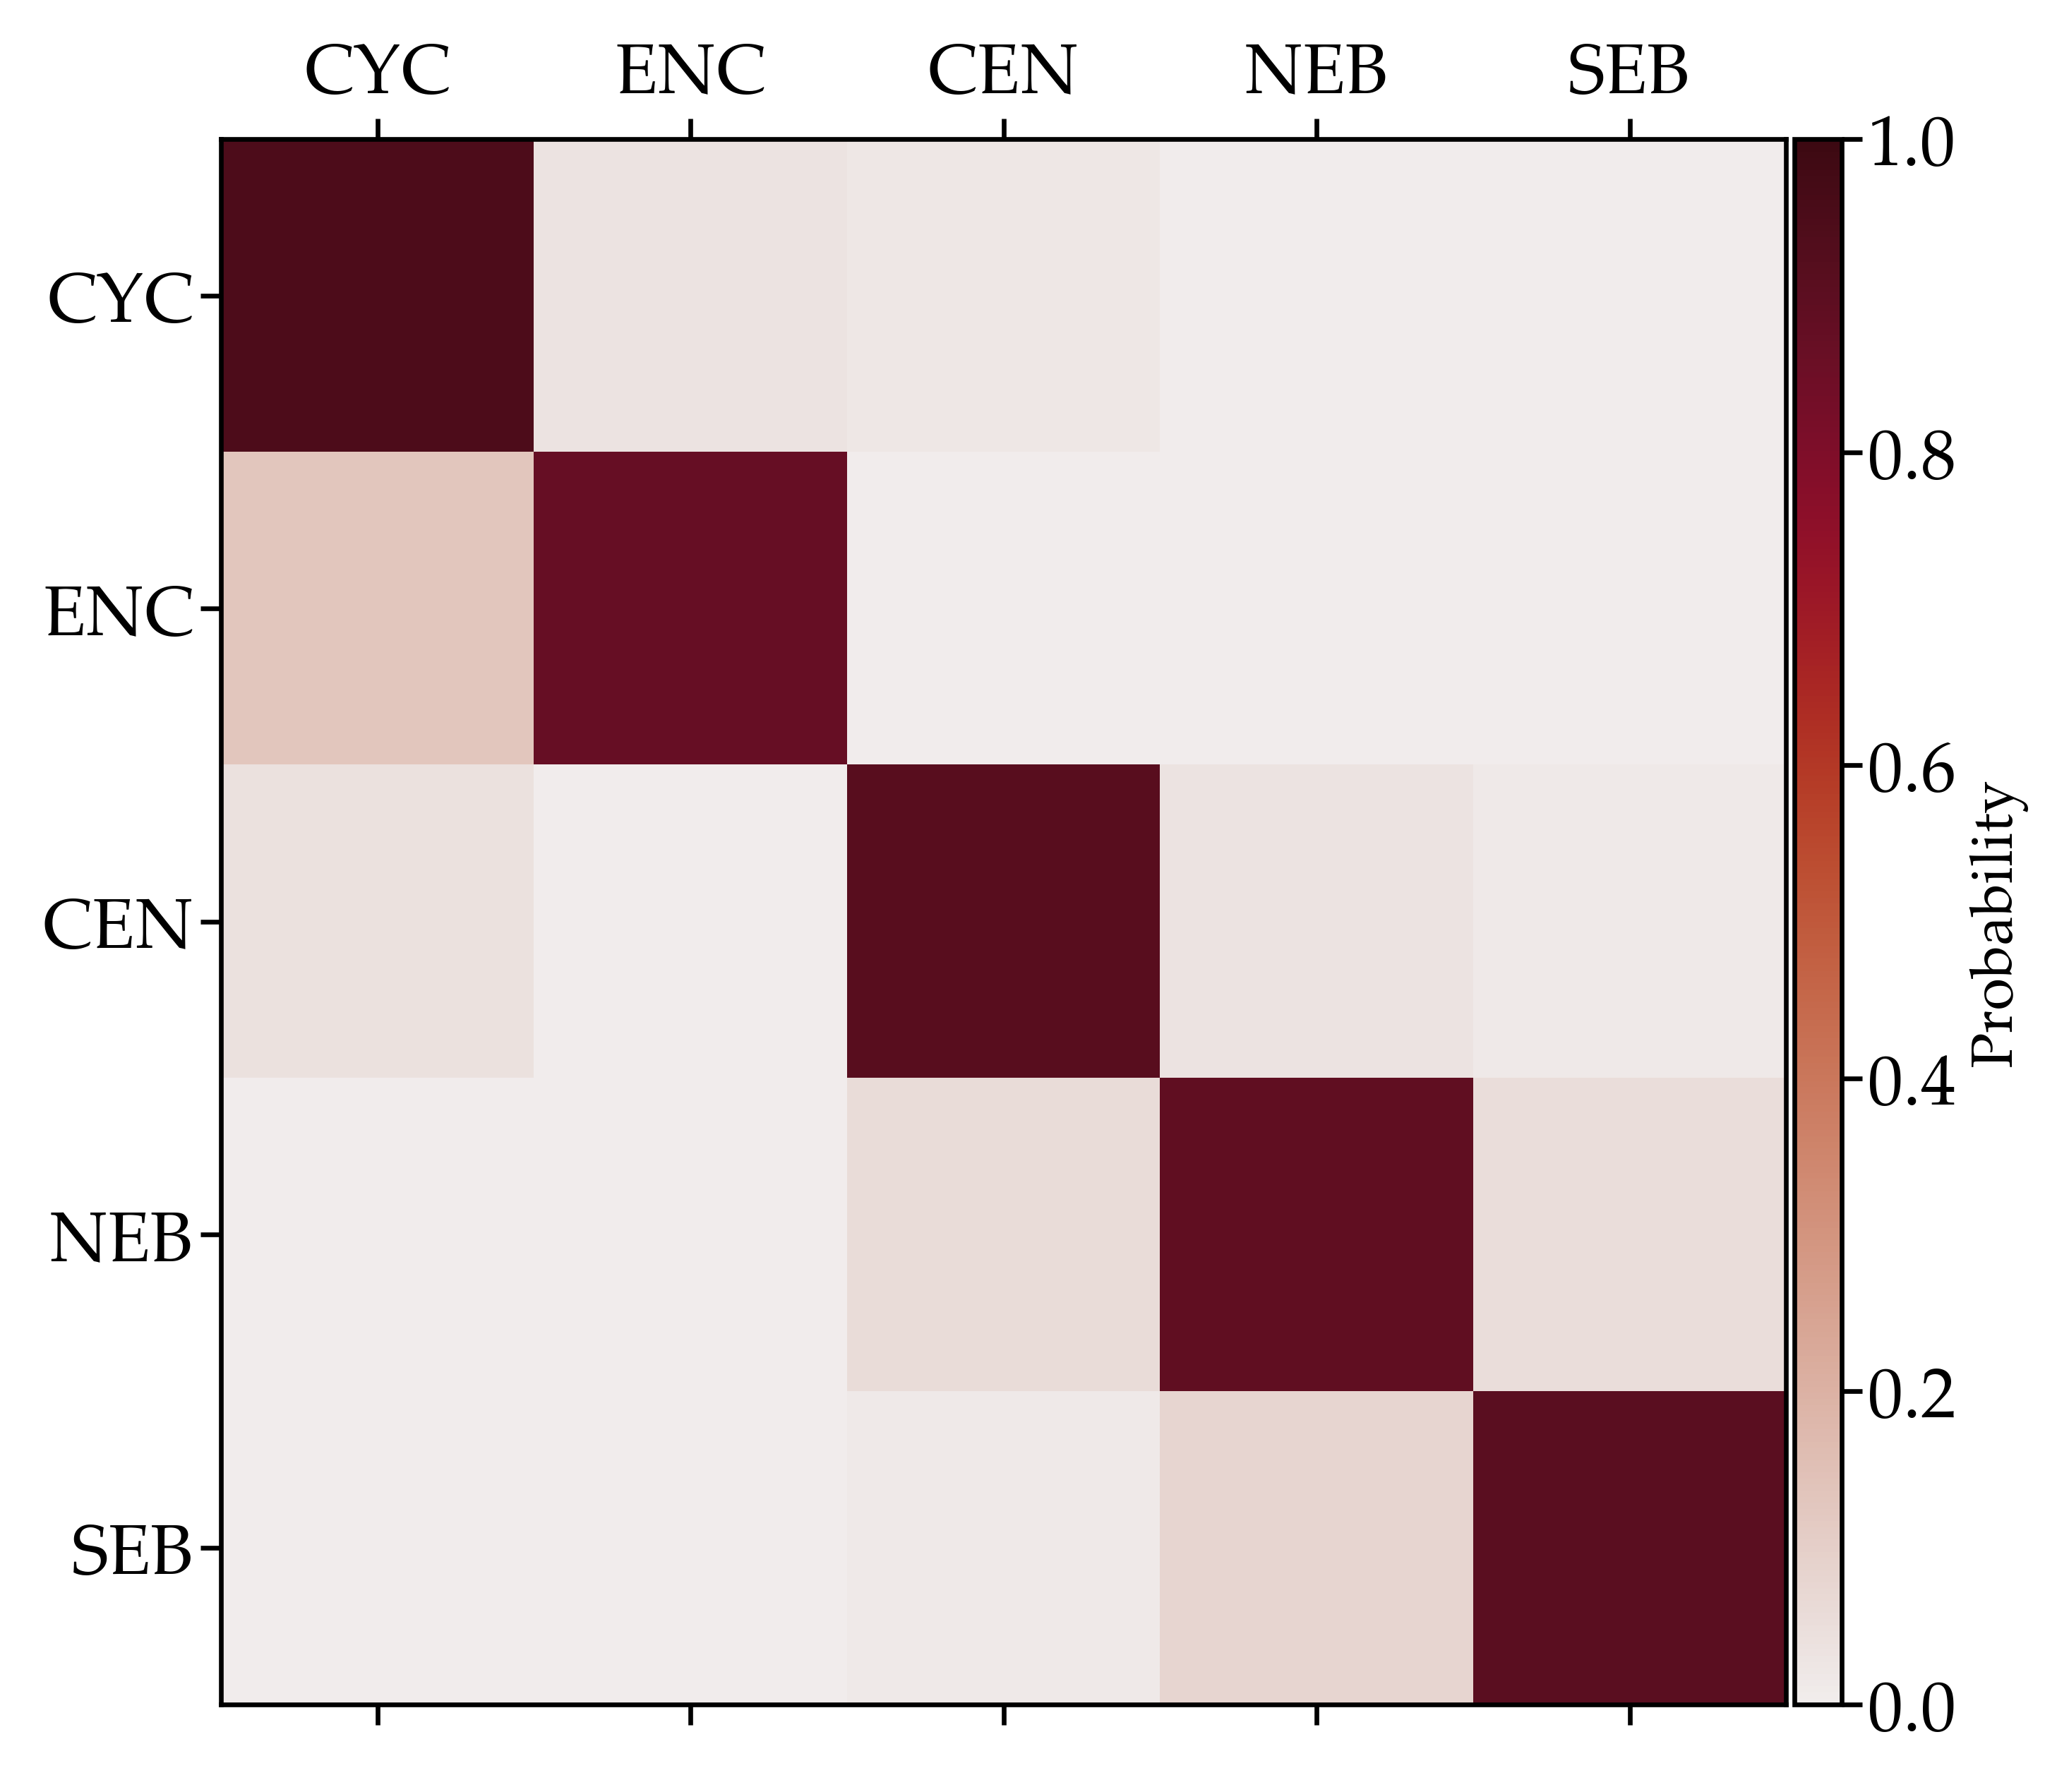
\includegraphics[width=0.9\textwidth]{1wconnection.png}
  }
  \only<2>{
  \frametitle{Connectivity matrix (2 weeks)}
  %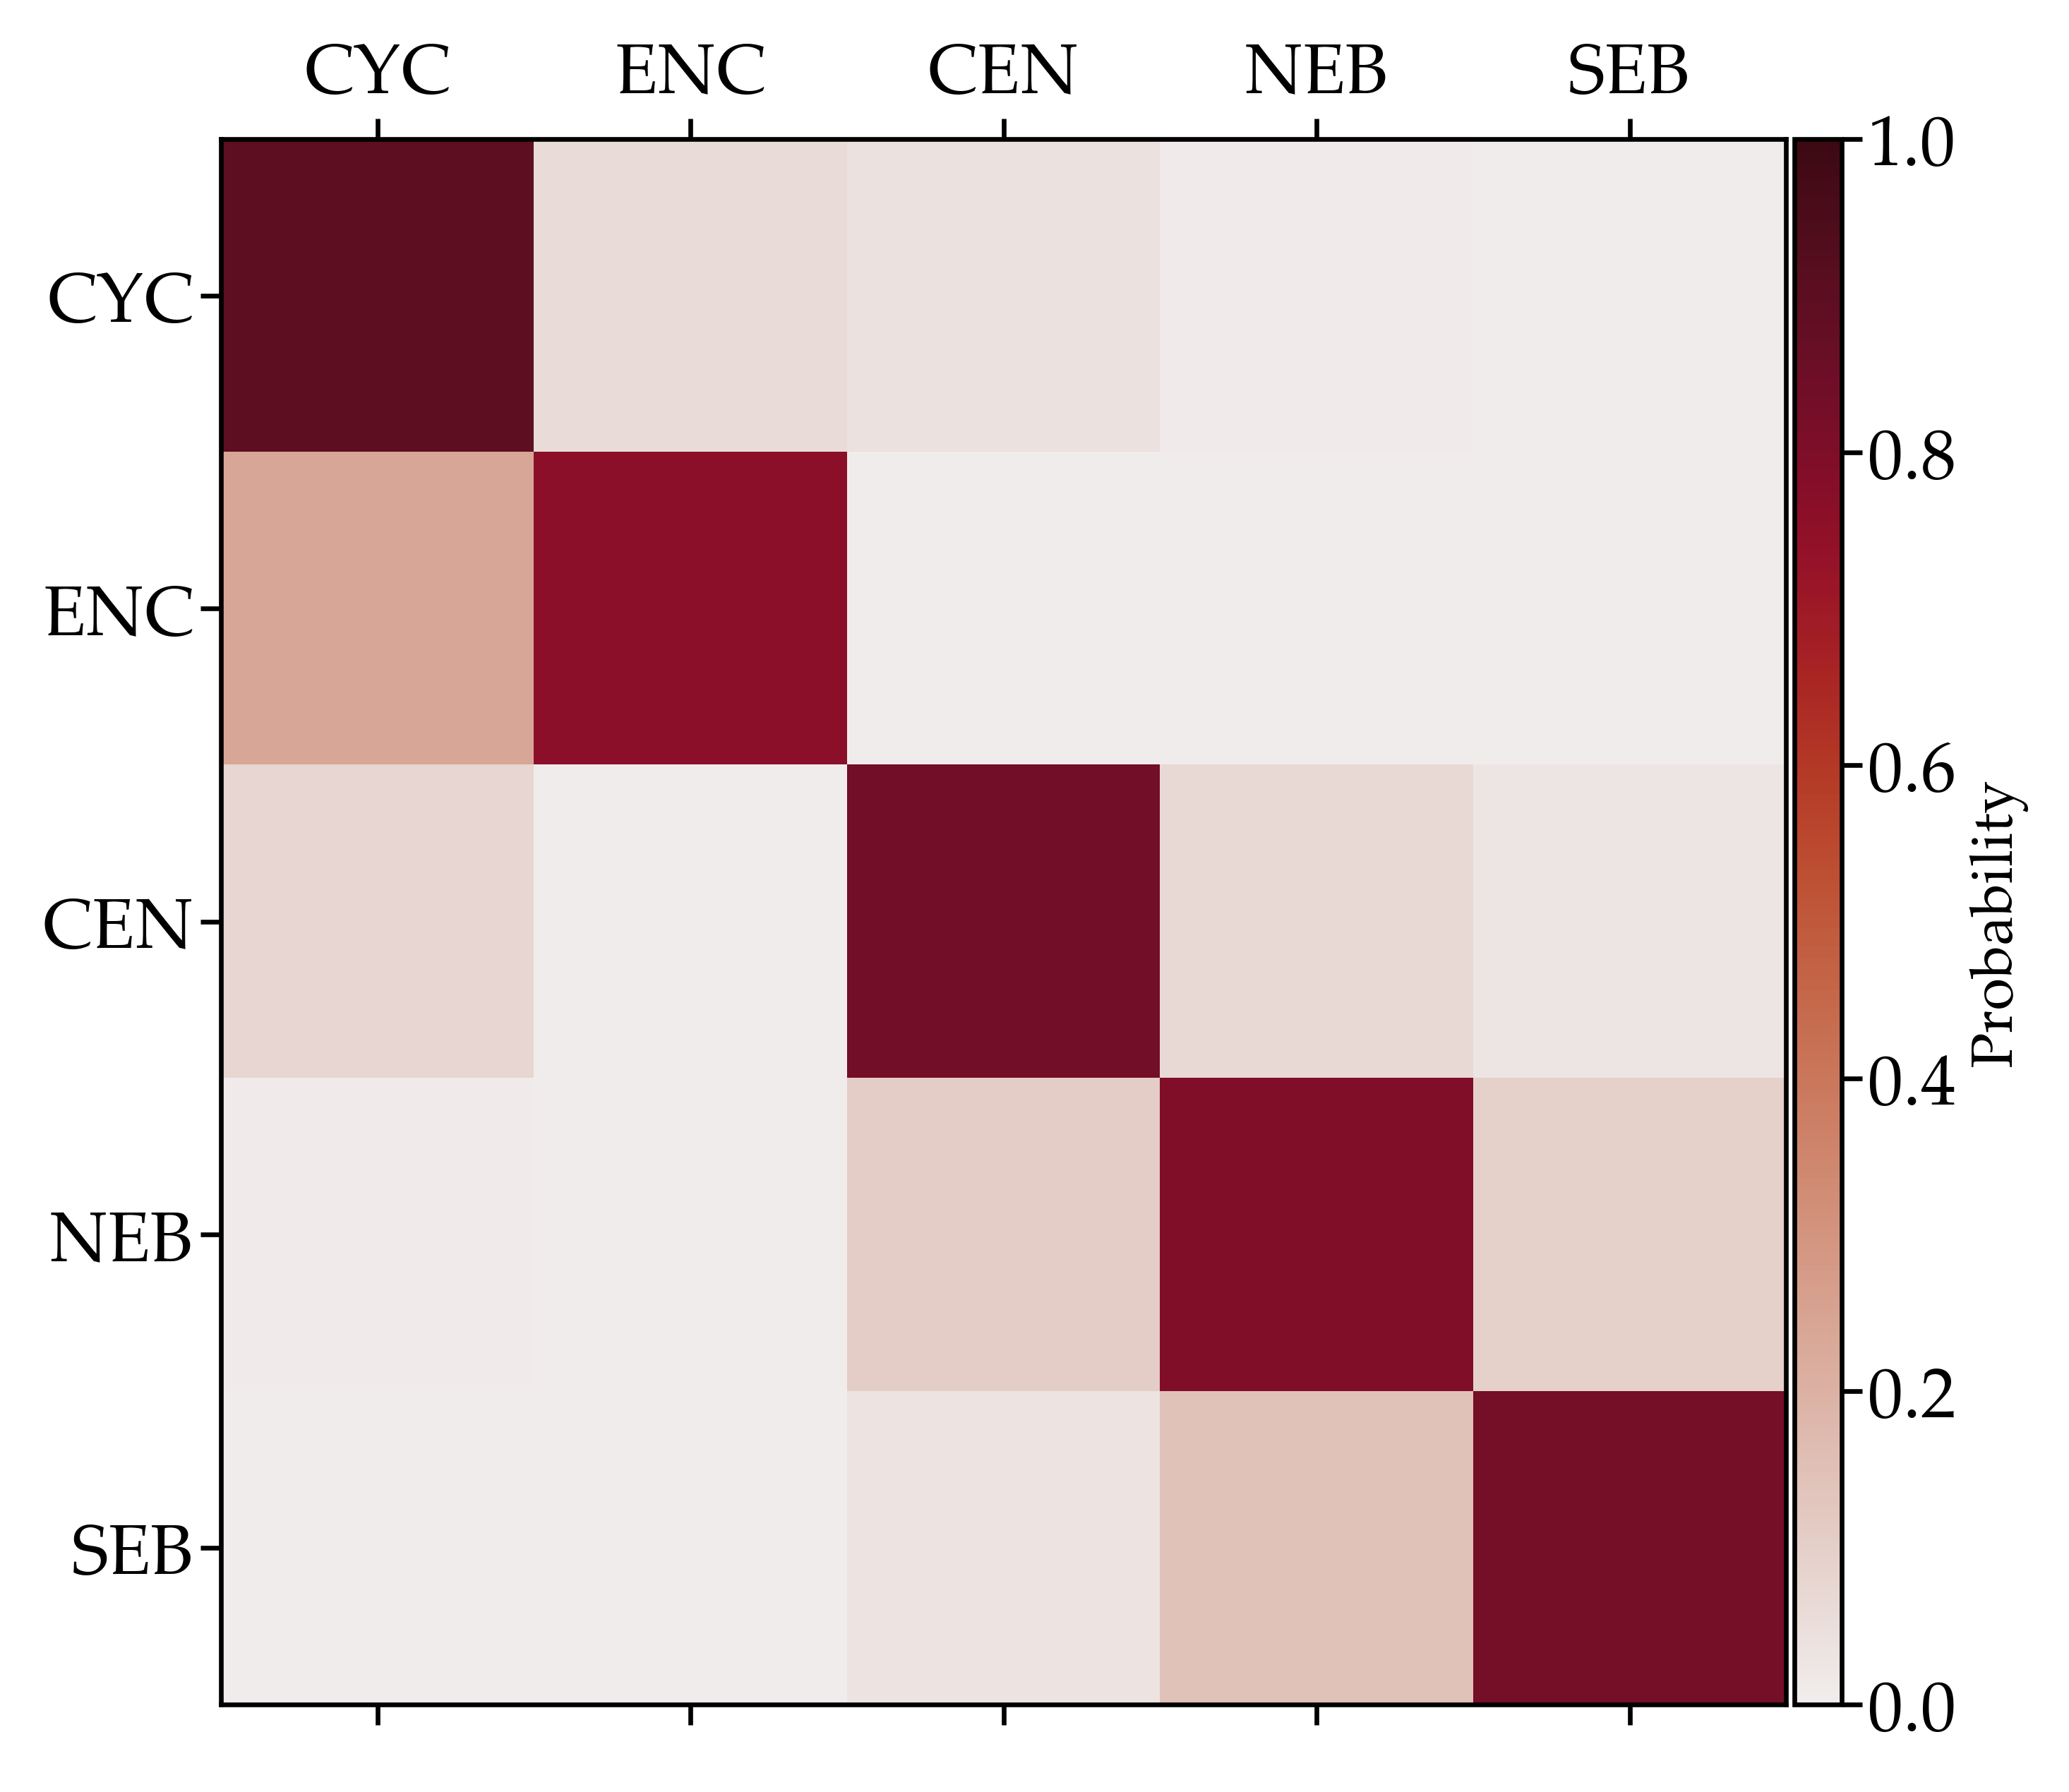
\includegraphics[width=0.9\textwidth]{2wconnection.png}
  }
  \only<3>{
  \frametitle{Connectivity matrix (4 weeks)}
  %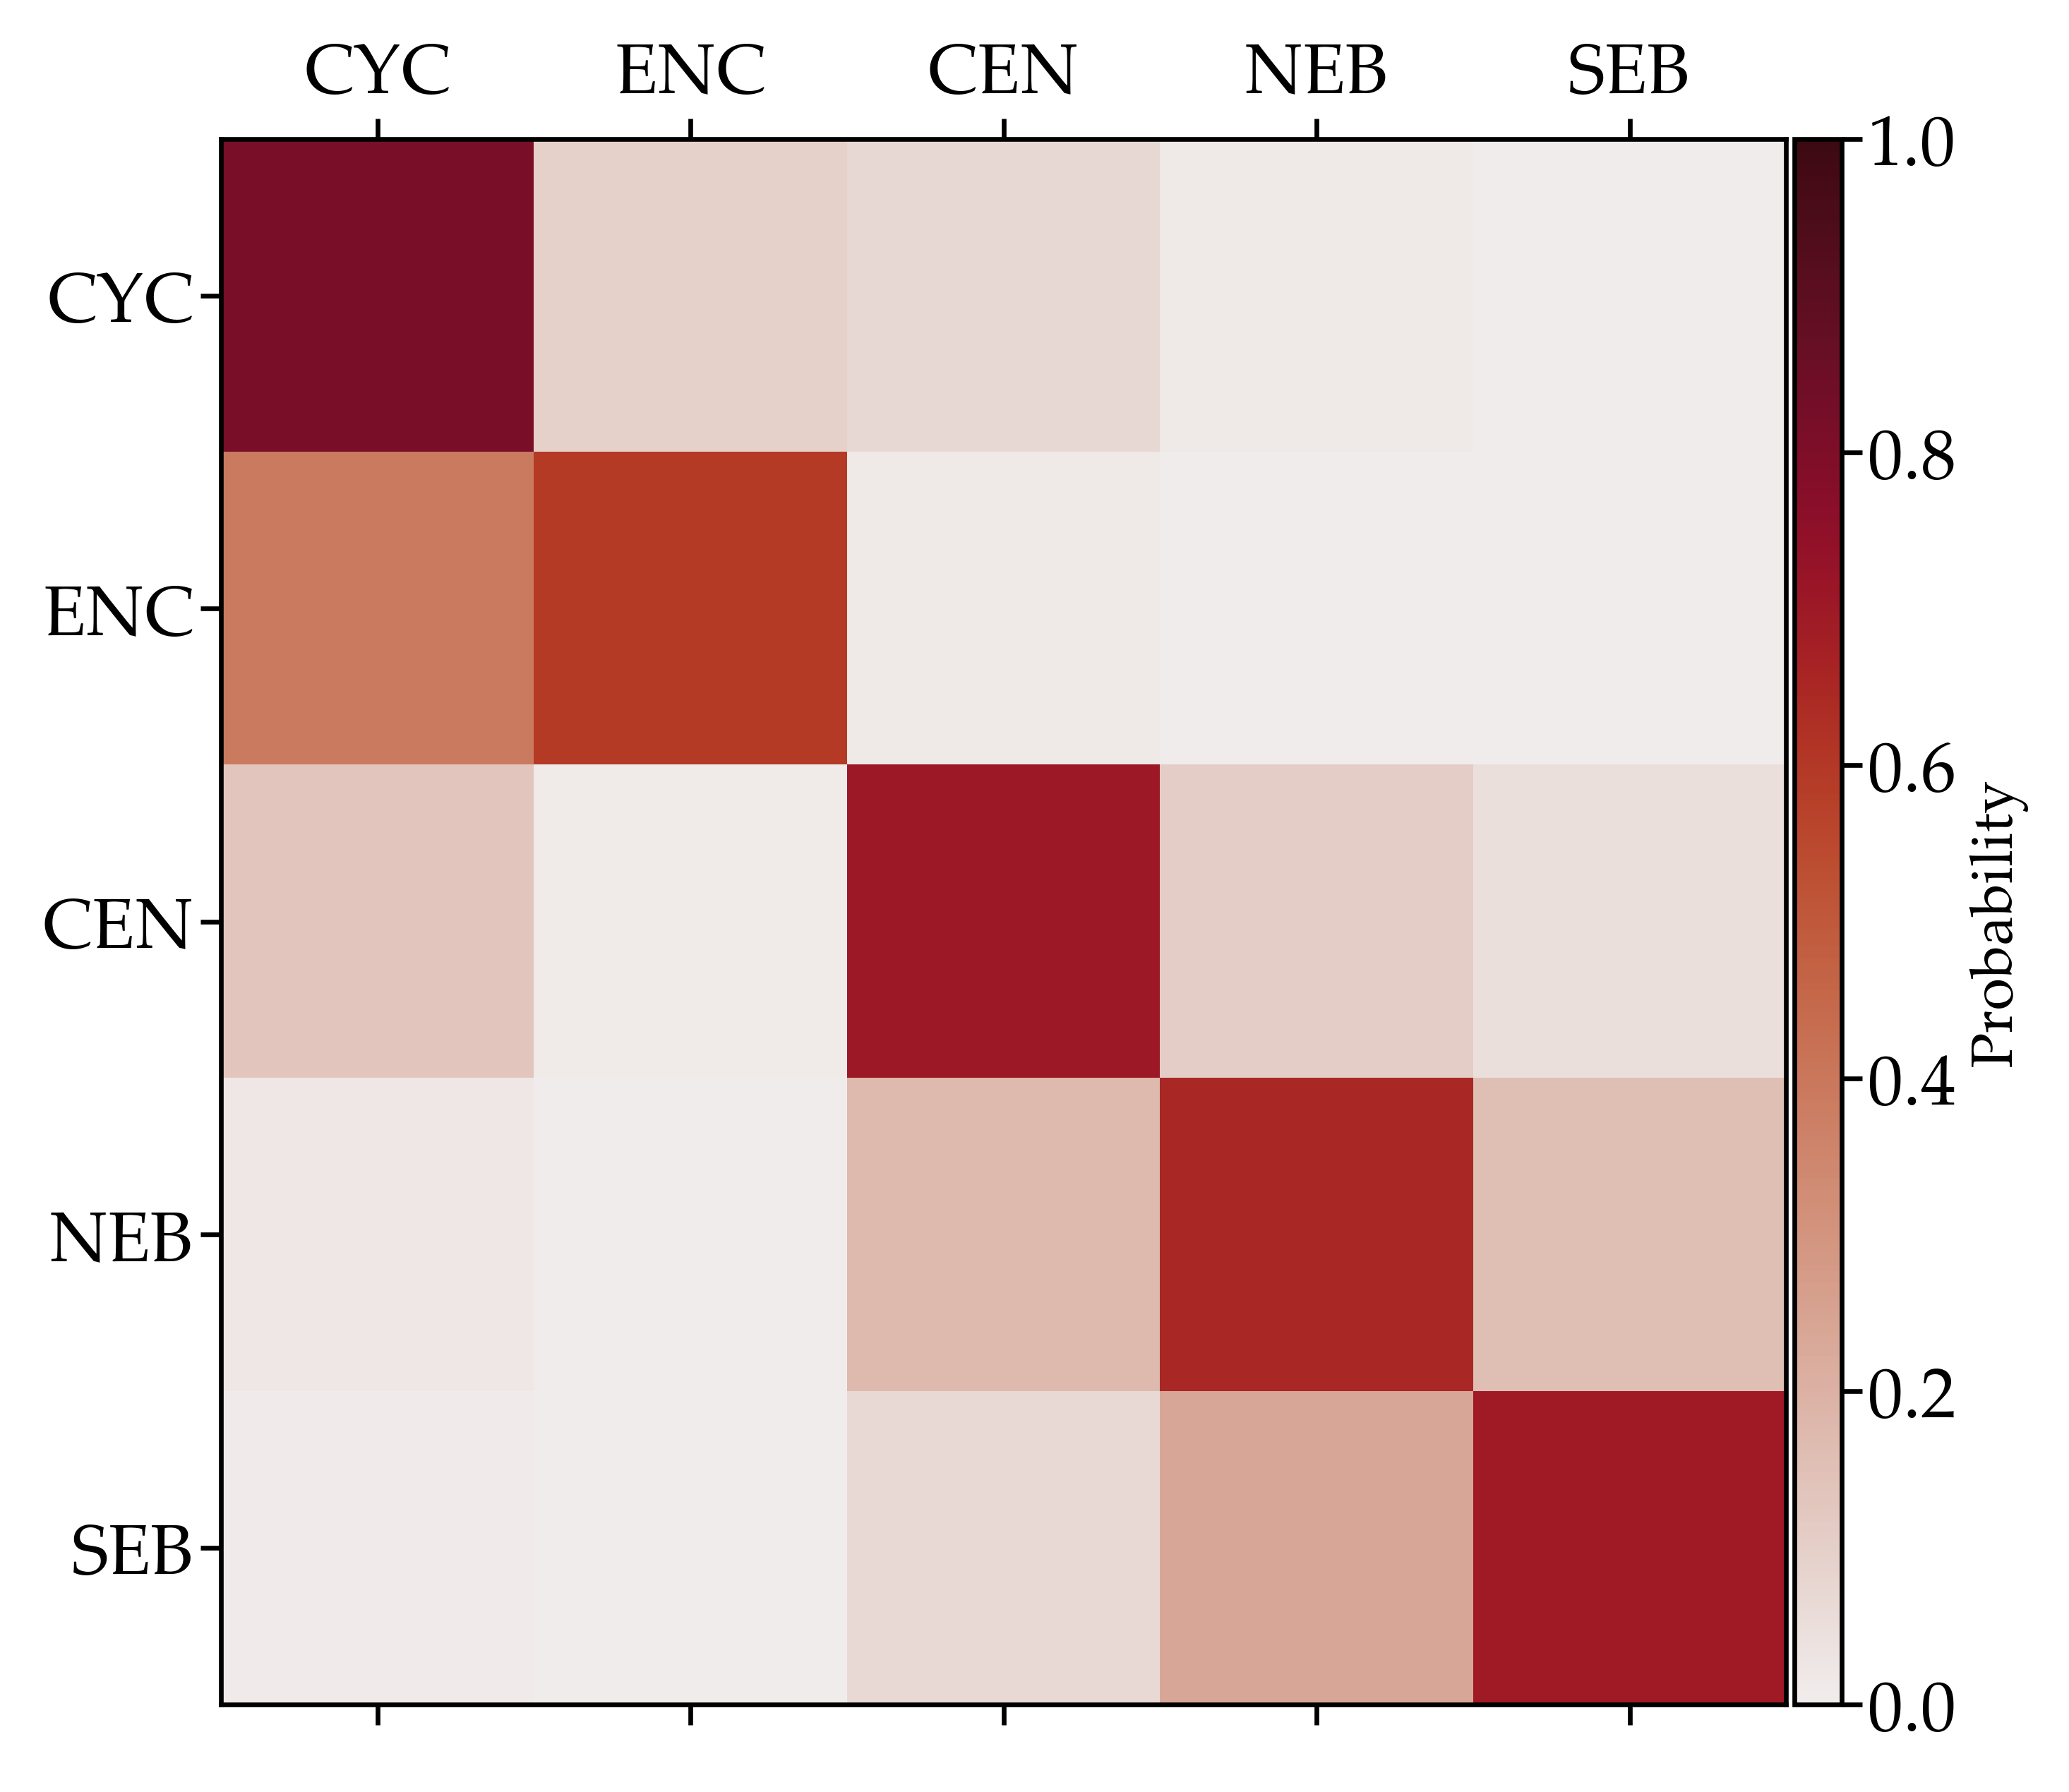
\includegraphics[width=0.9\textwidth]{4wconnection.png}
  }
\end{figure}
}


\frame{\frametitle{Residence time}
The time $\tau$ for a trajectory in box $B_i$ to move out of $A$, also known also as the mean time to hit the complement of $A$ \parencite{Norris-98}.
\begin{equation} 
  (\Id - P|_A)\tau/T = \mathbf{1},
\end{equation}
The time on average to reach a given province
starting from any province can be computed using \eqref{eq:tau} with $A$ set to the target province. We can see the cyclonic motion on the western region \parencite{Perez-etal-17}.
\begin{figure}
  %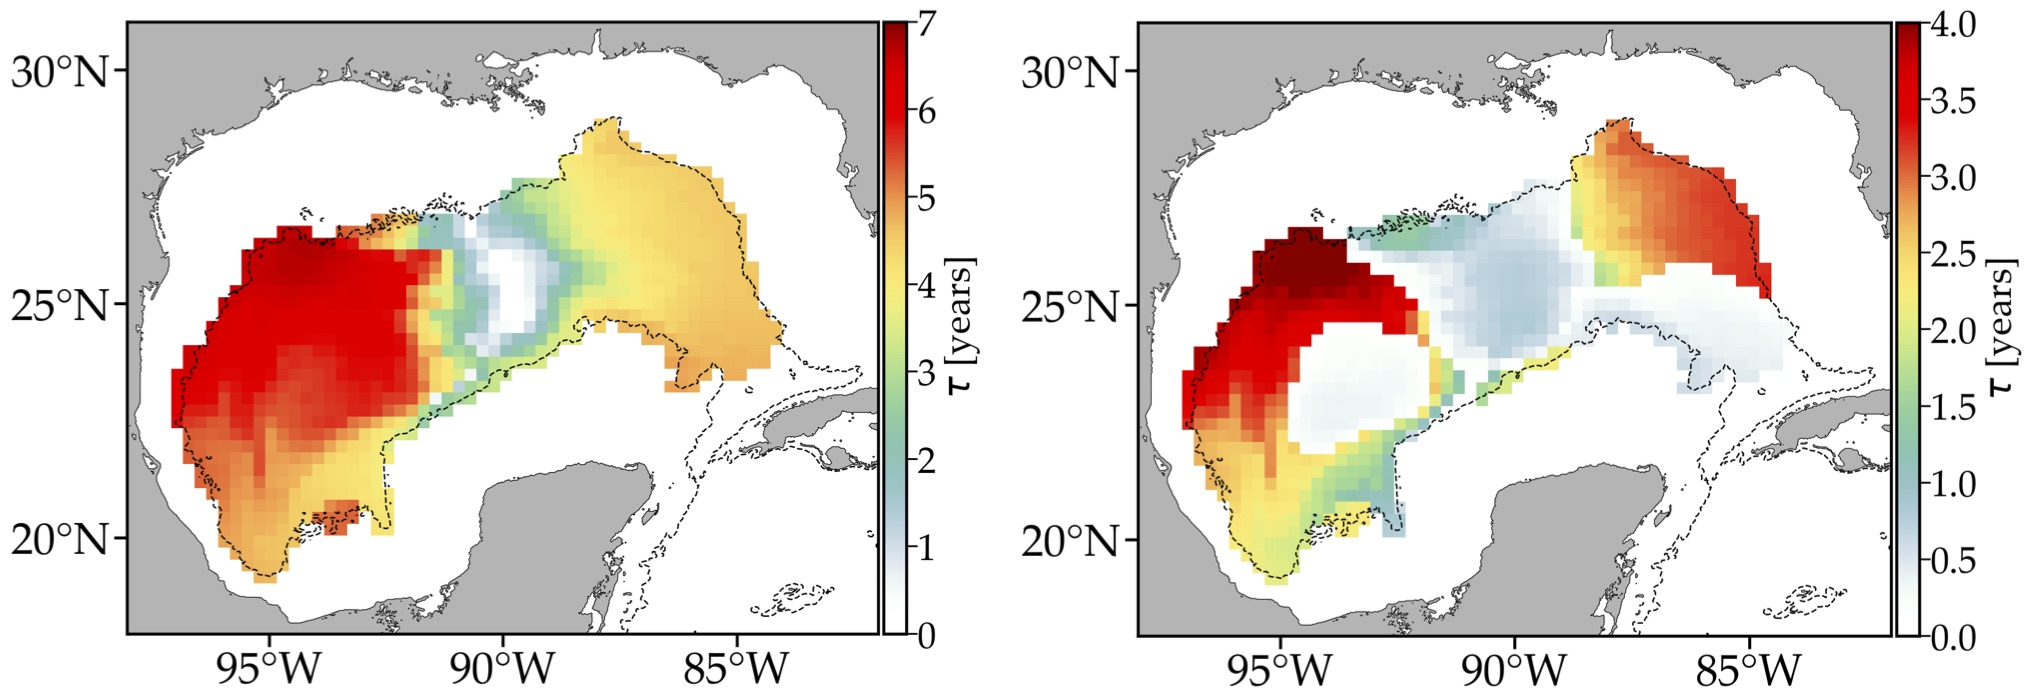
\includegraphics[width=\textwidth]{geogomdeep-figtau.jpg}
\end{figure}
}


\frame{\frametitle{Mean expected hitting time (complement of A in \eqref{eq:tau})}
\begin{figure}
    %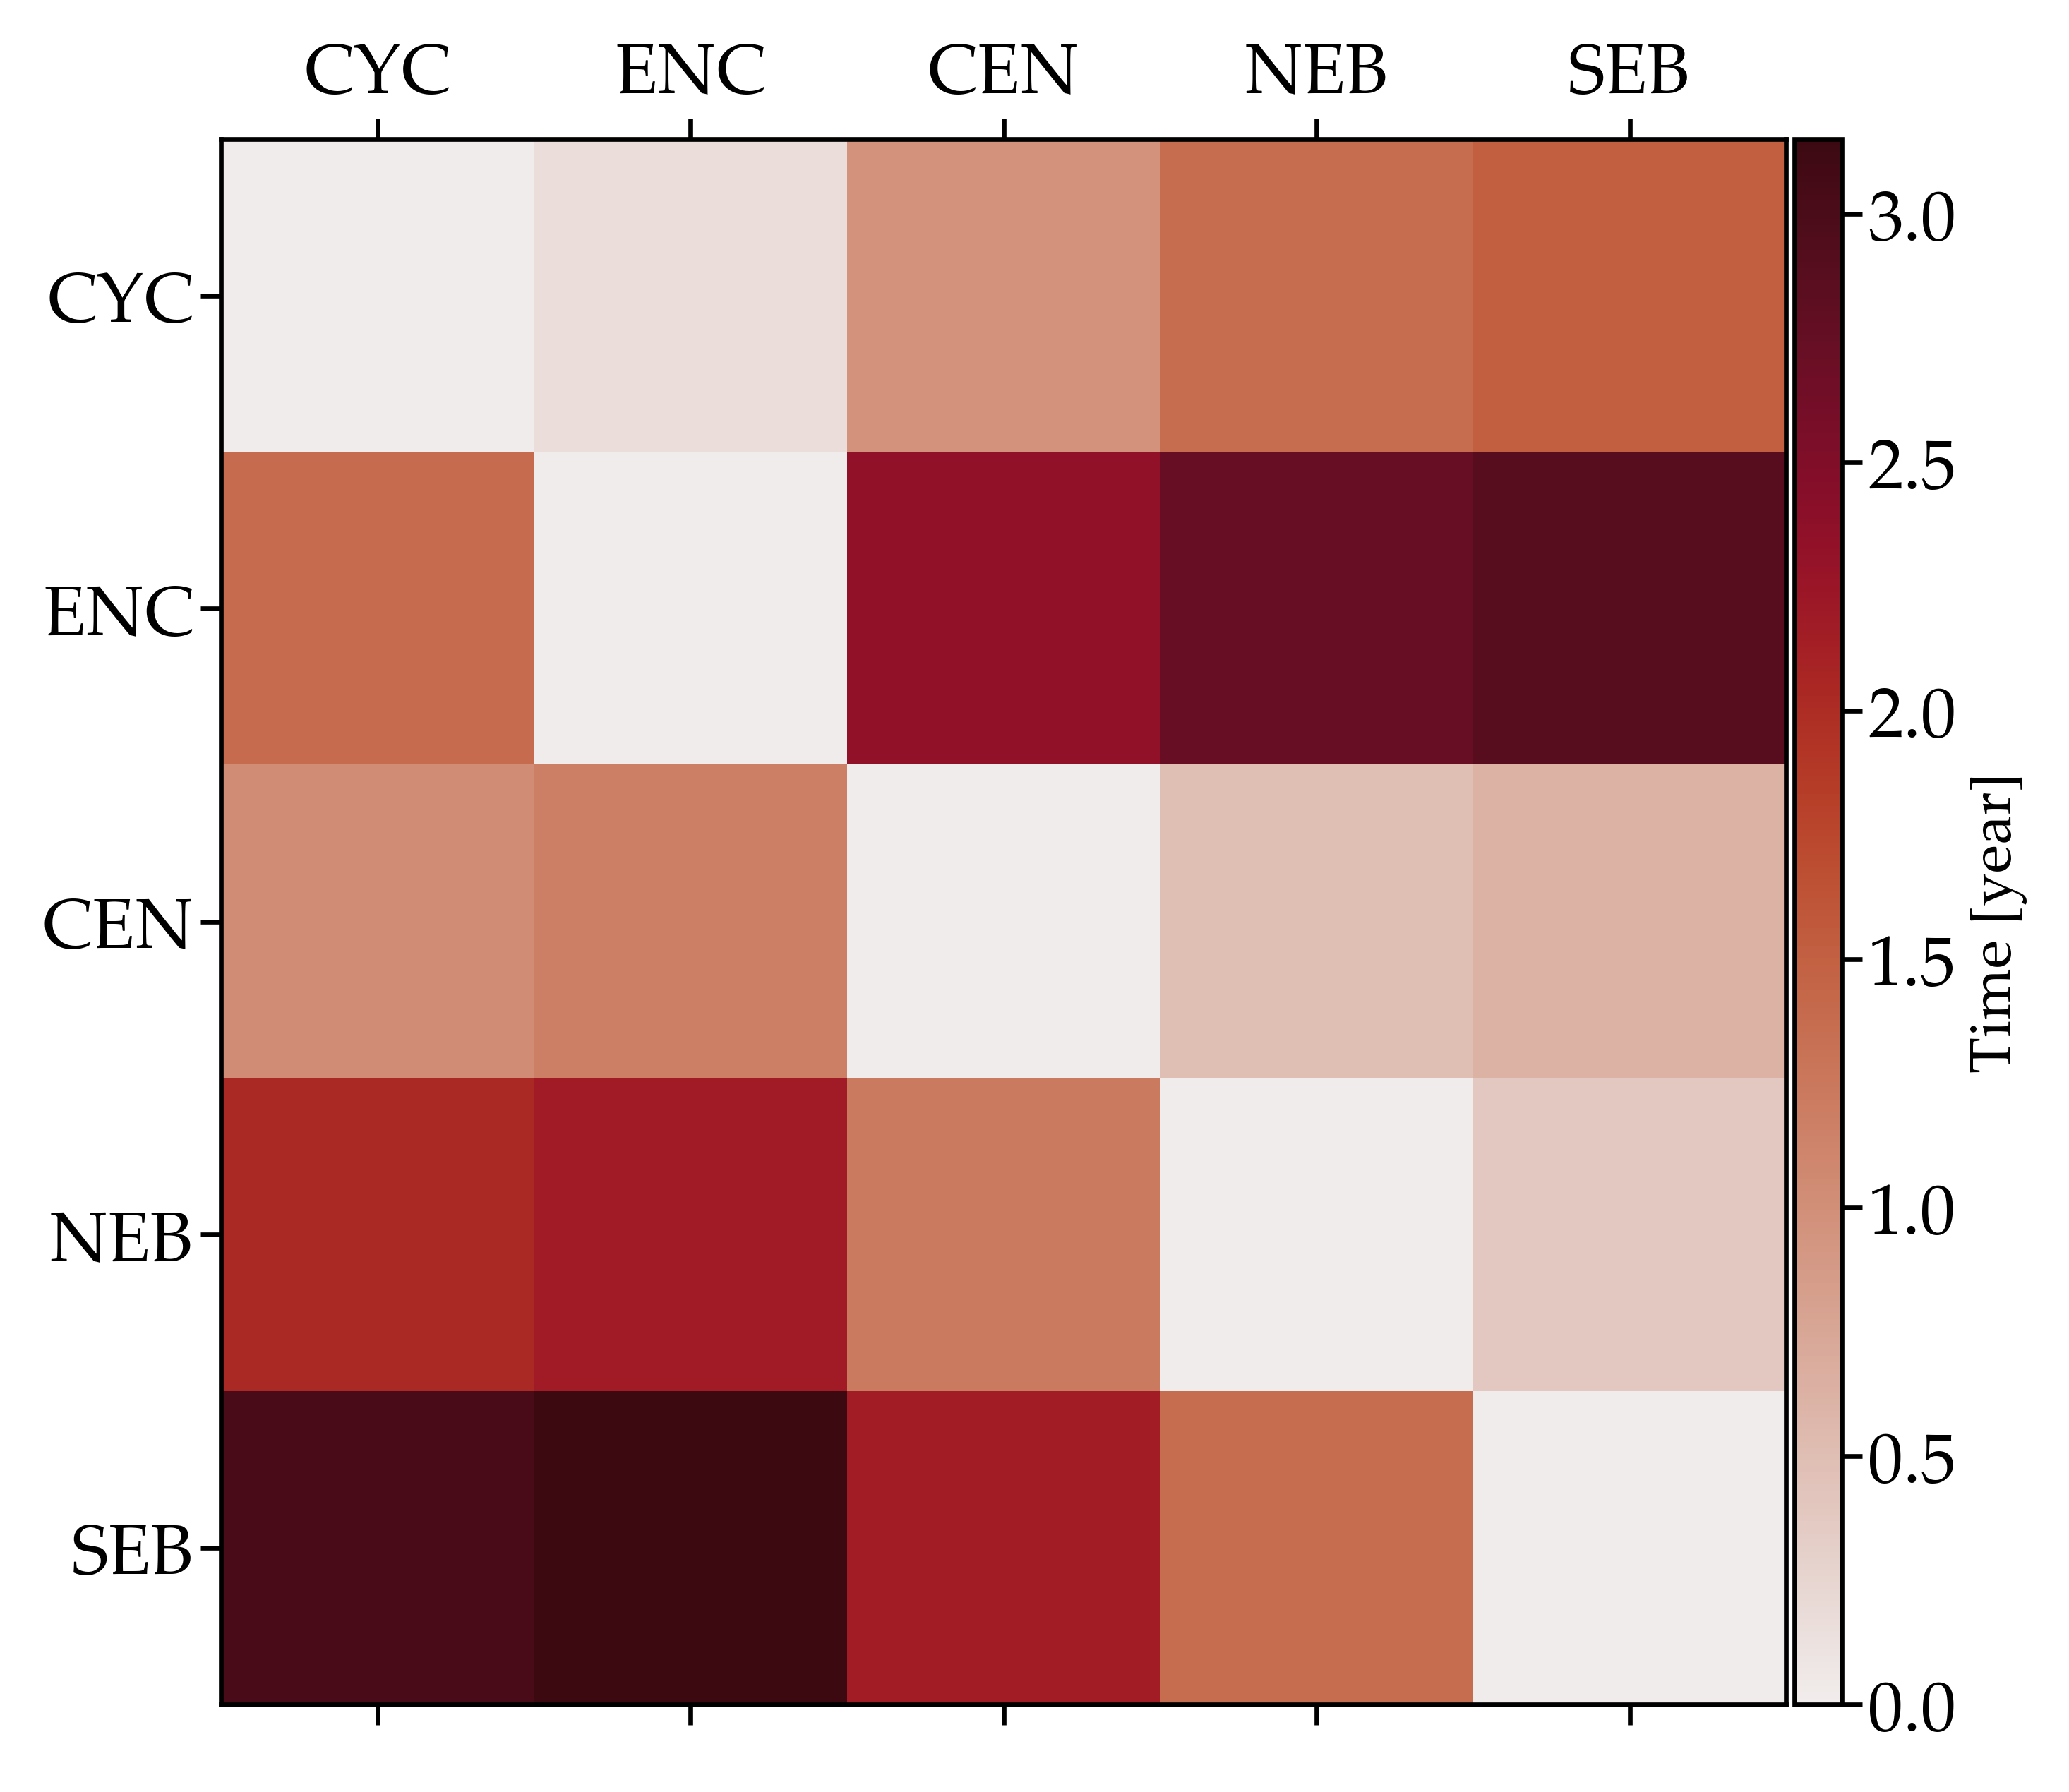
\includegraphics[width=0.9\textwidth]{hitting_time.png}
\end{figure}
}

\frame{\frametitle{Validation with experimental data \parencite{Ledwell-etal-16}}
Tracer mostly spreads along the continental slope and across Eastern bassin.
\begin{figure}
  \centering
  %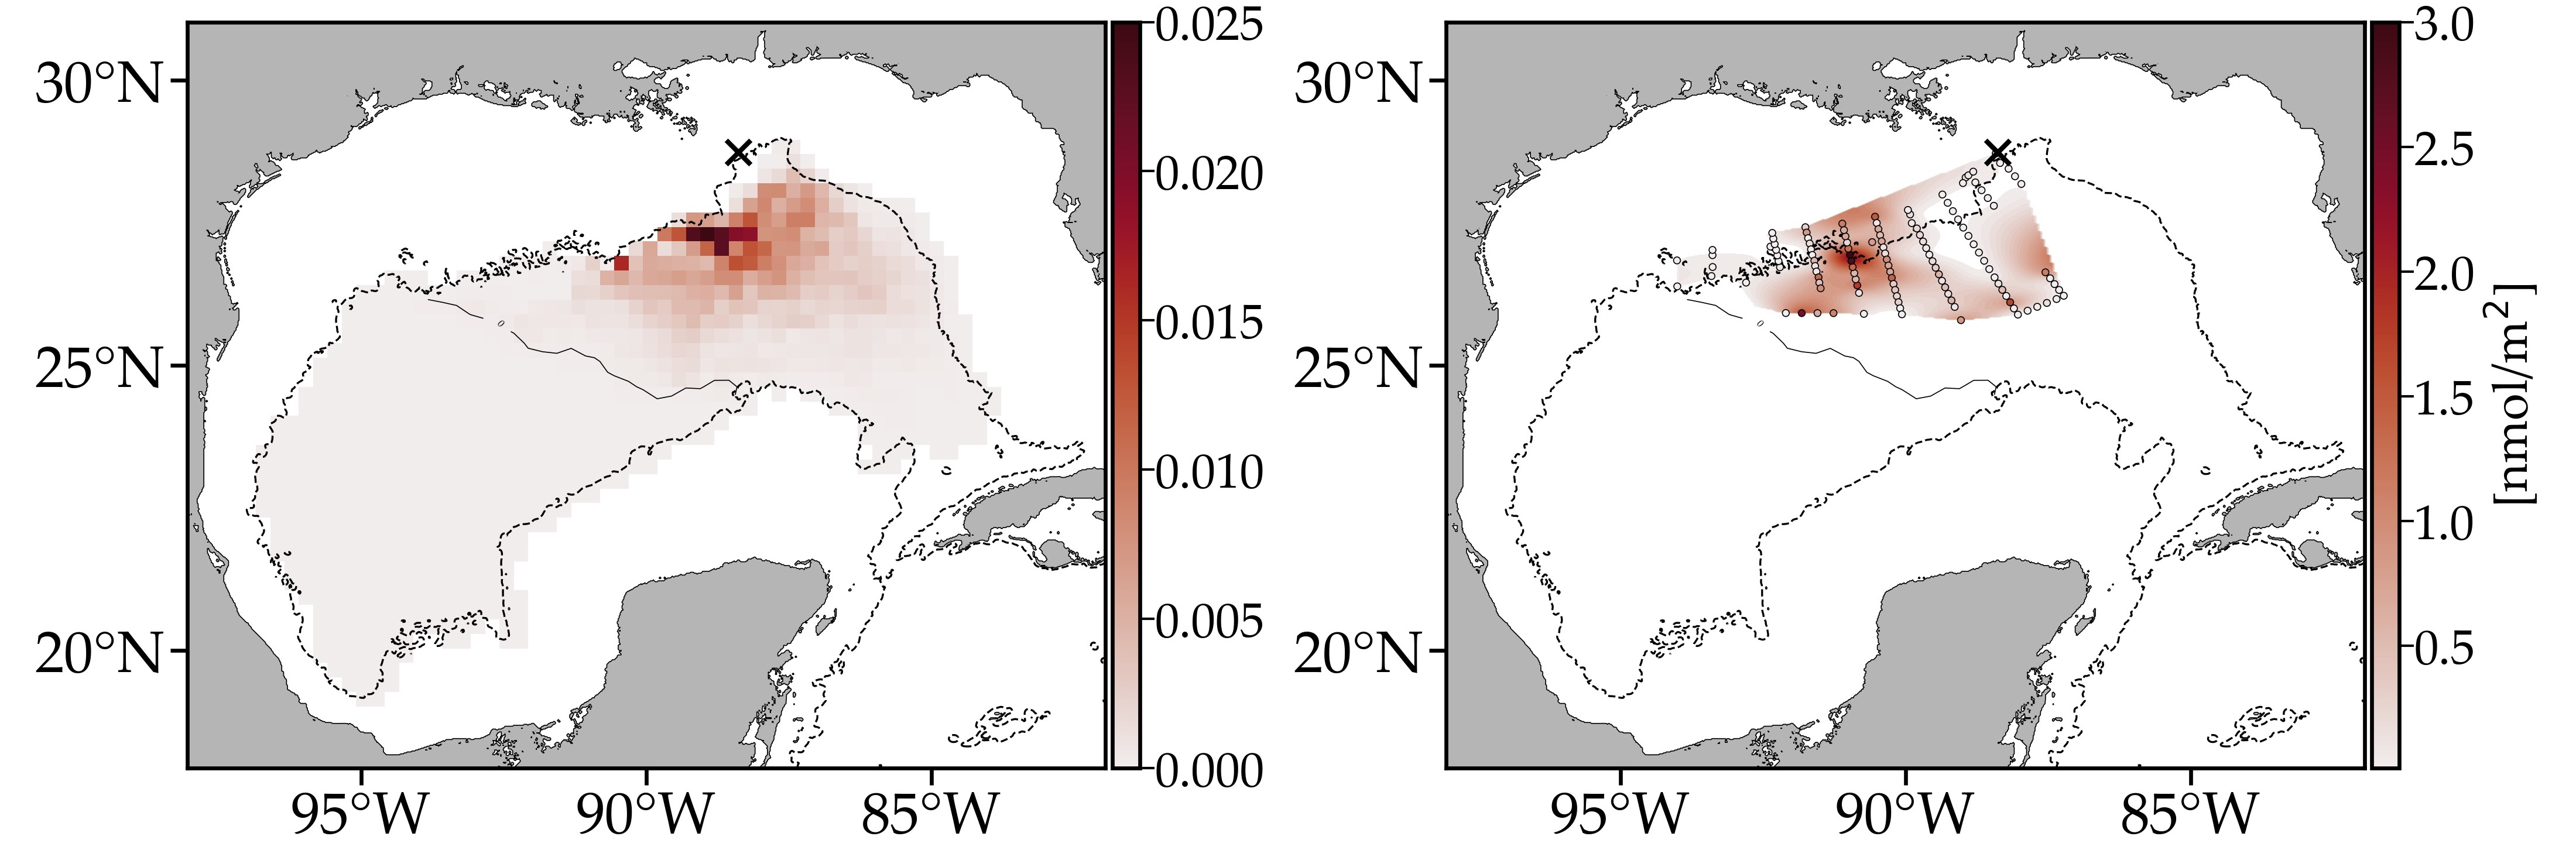
\includegraphics[width=1\textwidth]{geogomdeep-fig11.jpg}
  
  %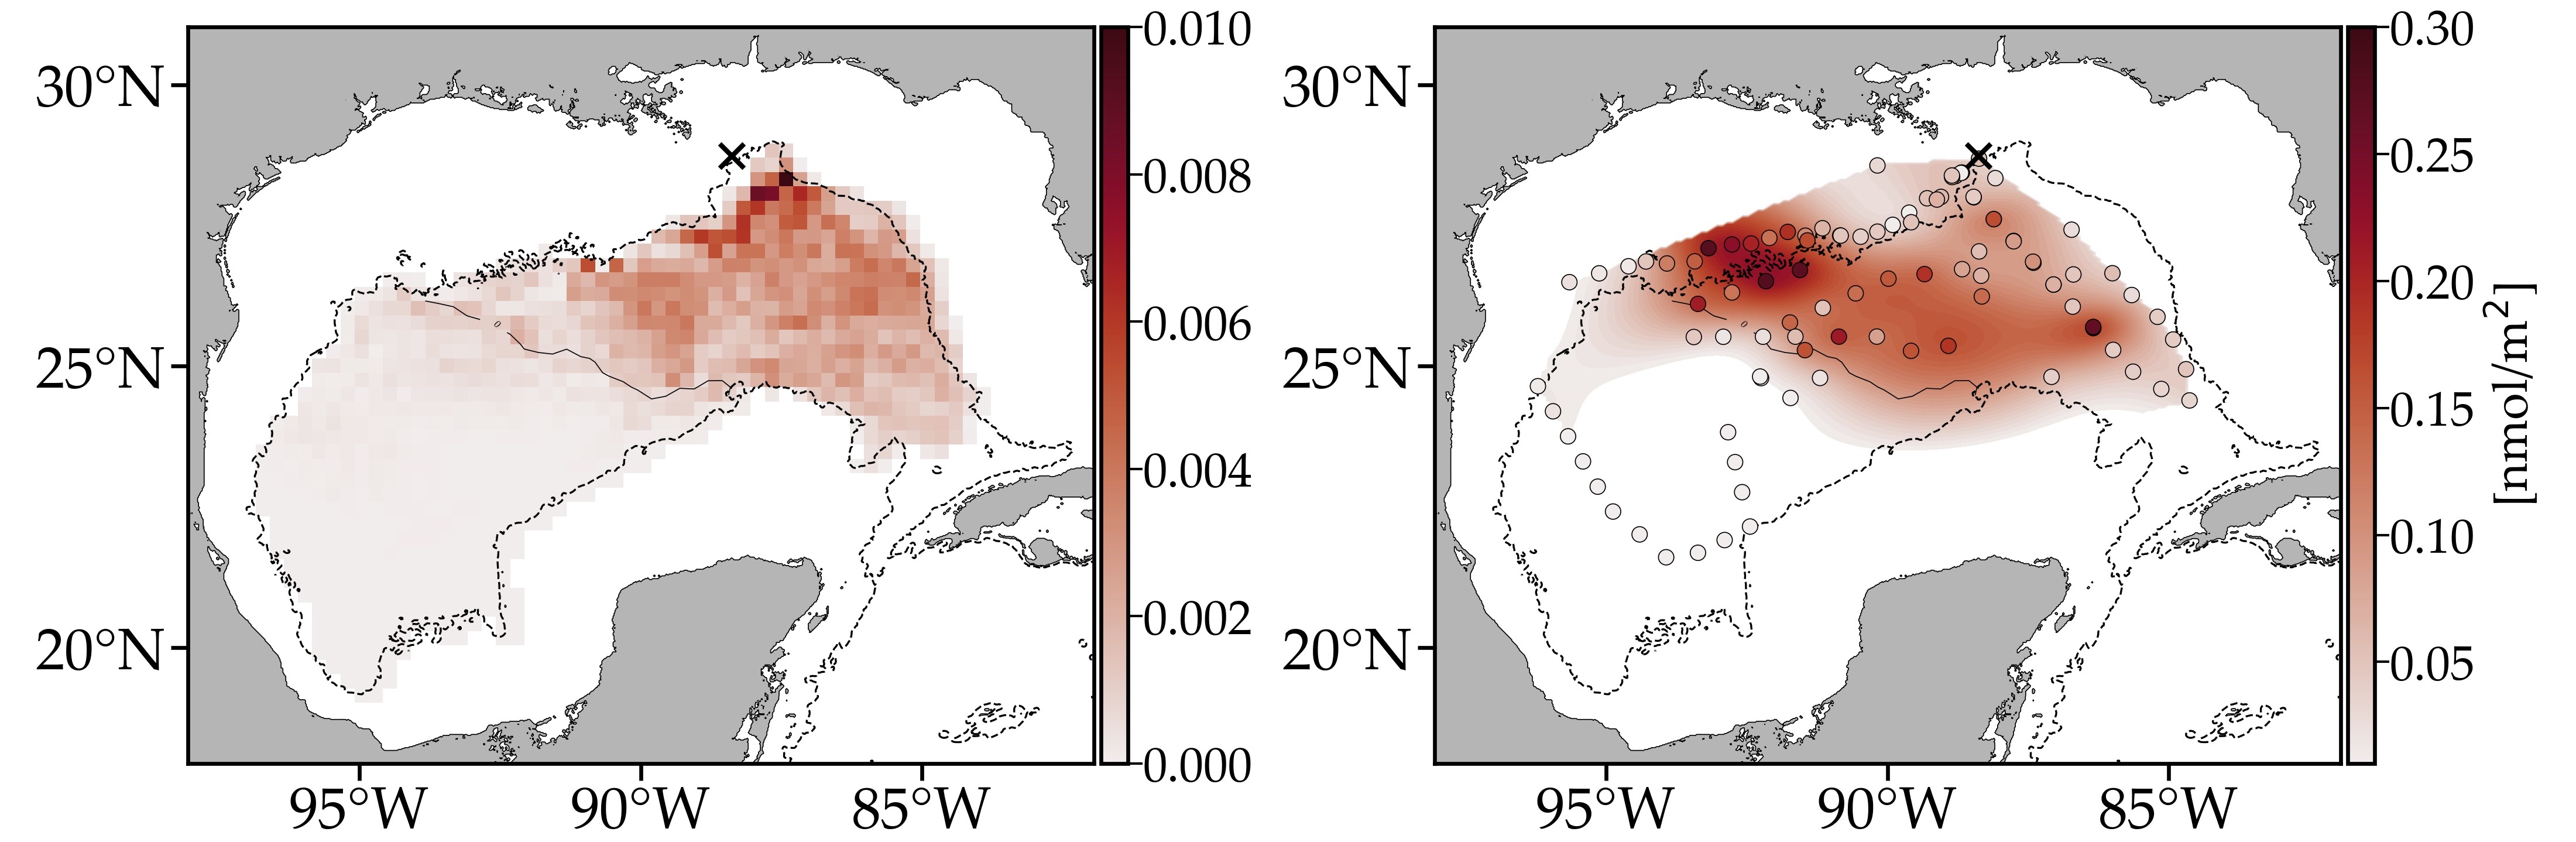
\includegraphics[width=1\textwidth]{geogomdeep-fig11b.jpg}
\end{figure}
}



% -----------------------
% second part of the talk
% -----------------------
\title{Markov-chain-inspired search for MH370}
\author{P. Miron\inst{1}, F.J. Beron-Vera\inst{1}, M.J. Olascoaga\inst{1}, P. Koltai\inst{2}}
\institute % (optional, but mostly needed)
{
  \inst{1}%
  Rosenstiel School of Marine and Atmospheric Science\\
  University of Miami
  \and
  \inst{2}%
  Institute of Mathematics, Freie Universit\"at\\
  Berlin, Berlin, Germany
}

\frame[plain,noframenumbering]{
\titlepage
}

%\begin{frame}{Outline}
%  \tableofcontents
  % You might wish to add the option [pausesections]
%\end{frame}

% Section and subsections will appear in the presentation overview
% and table of contents.
\section{Introduction}

\begin{frame}{Catastrophe}

The disappearance in the Indian ocean of Malaysian Airlines flight MH370 is one of the biggest aviation mysteries.

\begin{itemize}
	\item second deadliest incident involving a Boeing 777 (227 passengers and 12 crew members) 
	\item most expensive search in aviation history (\$155 million)
	\begin{itemize}
		\item 2 years and 4 months
    	\item 4 vessels equipped with deep-water vehicles, sonars and cameras
  		\item underwater scan of a 120 000 km$^2$ search area
    \end{itemize}
 \end{itemize}
\end{frame}

\begin{frame}{Time of March 8, 2014  (UTC time)}
\begin{itemize}
	\item 16:42: takeoff from KUL to PEK with an expected arrival 22:30 (00:42--06:30\,MYT)
	\item 17:06: aircraft final transmission (position and remaining fuel)
	\item 17:19: last verbal communication from the pilot to air traffic control
	\item 17:22--18:22: aircraft is observed by civilian and military radar until the transponder stopped working (or turned off)
	\item 19:41--00:19: seven log-on acknowledgements between the plane and the satellite
	\item 01:15: aircraft did not respond to a status request
\end{itemize}

23:24 (07:24\,MYT): Malaysia Airlines stated that contact with the plane was lost at 17:21 and that search operations were launched.
\end{frame}

\begin{frame}{Path reconstruction from the satellite \textit{ping} signal}
\begin{figure}[hbt]
  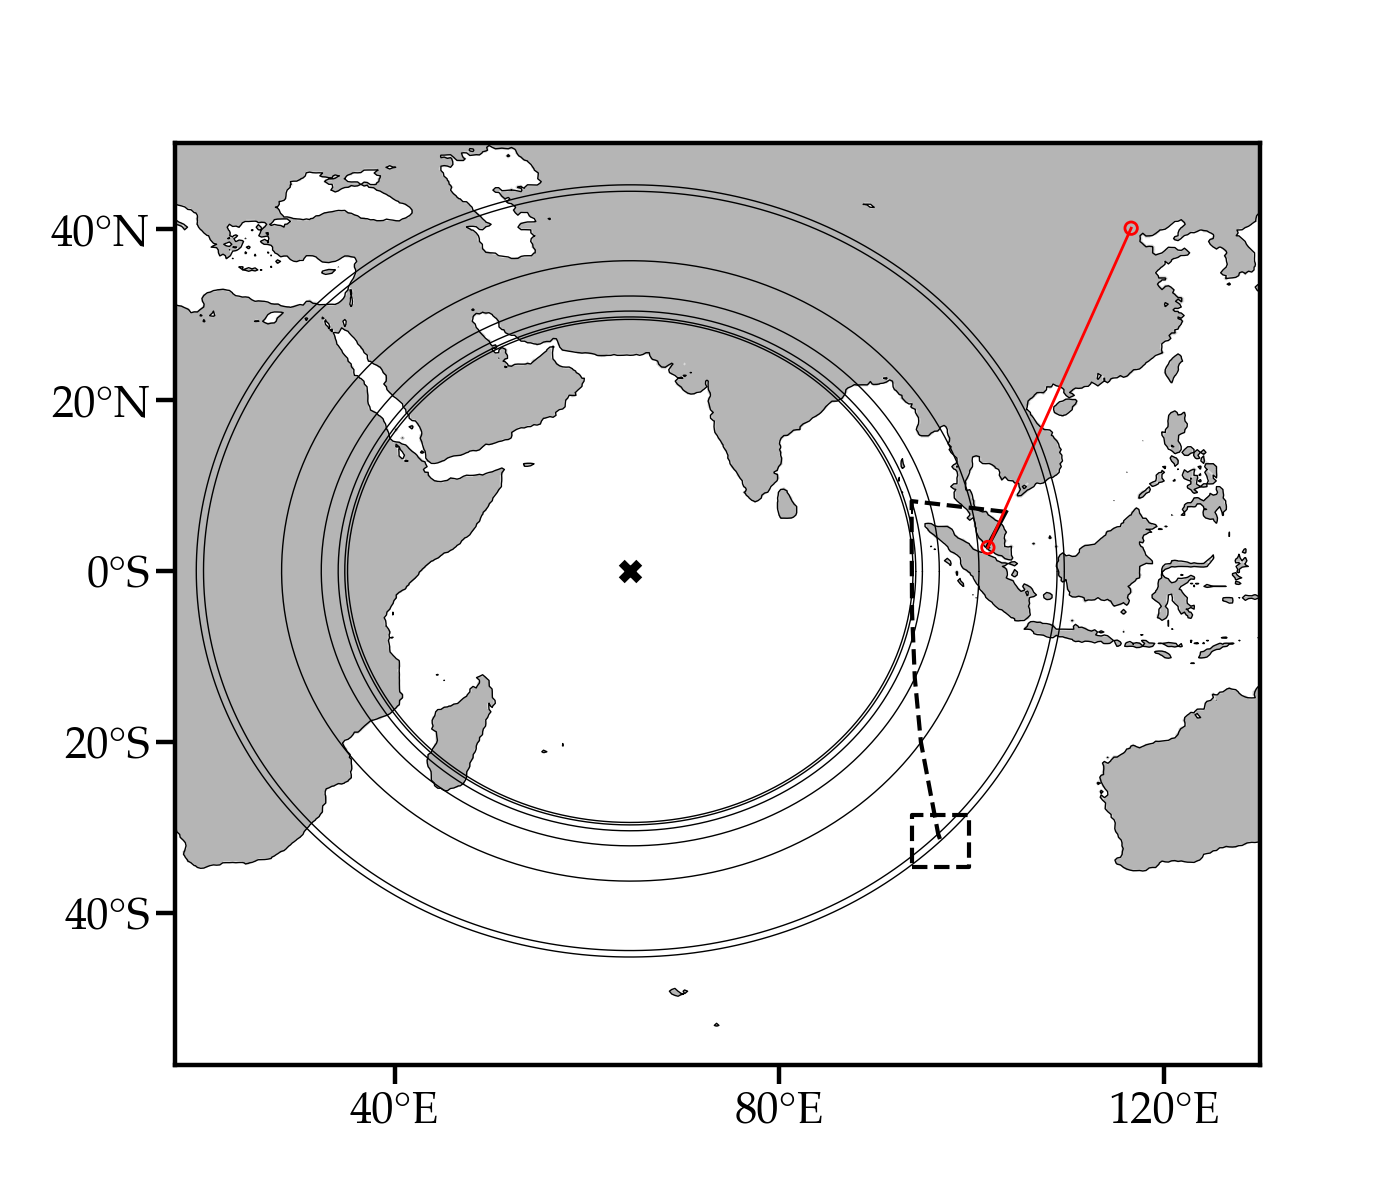
\includegraphics[width=0.85\textwidth]{figures/arcs_map.png}
\end{figure}
\end{frame}

\begin{frame}{First debris reached Reunion Island}

\begin{figure}[hbt]
  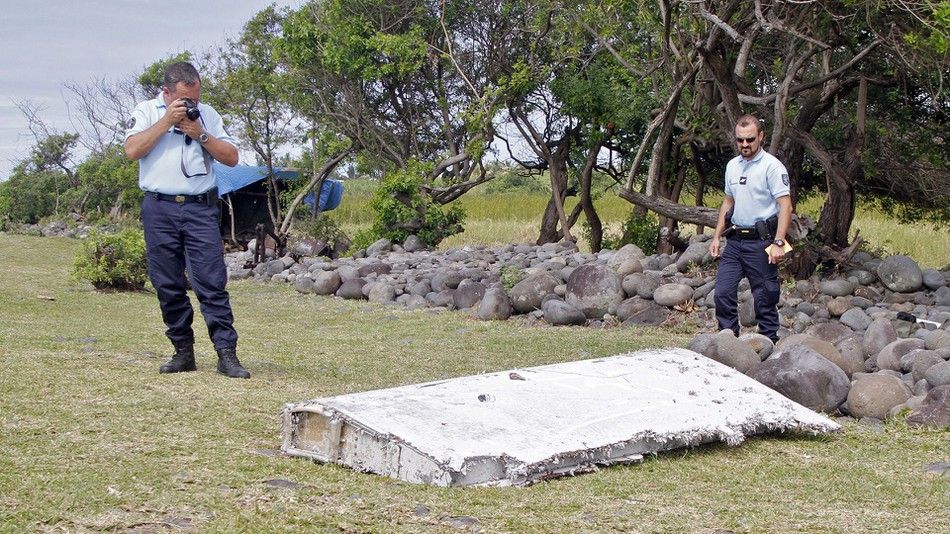
\includegraphics[width=\textwidth]{figures/flaperon.jpg}
  \caption{508 days after the crash of the airplane}
\end{figure}

\end{frame}

\begin{frame}{Confirmed debris beachings (508--838 days)}  

\begin{figure}[hbt]
  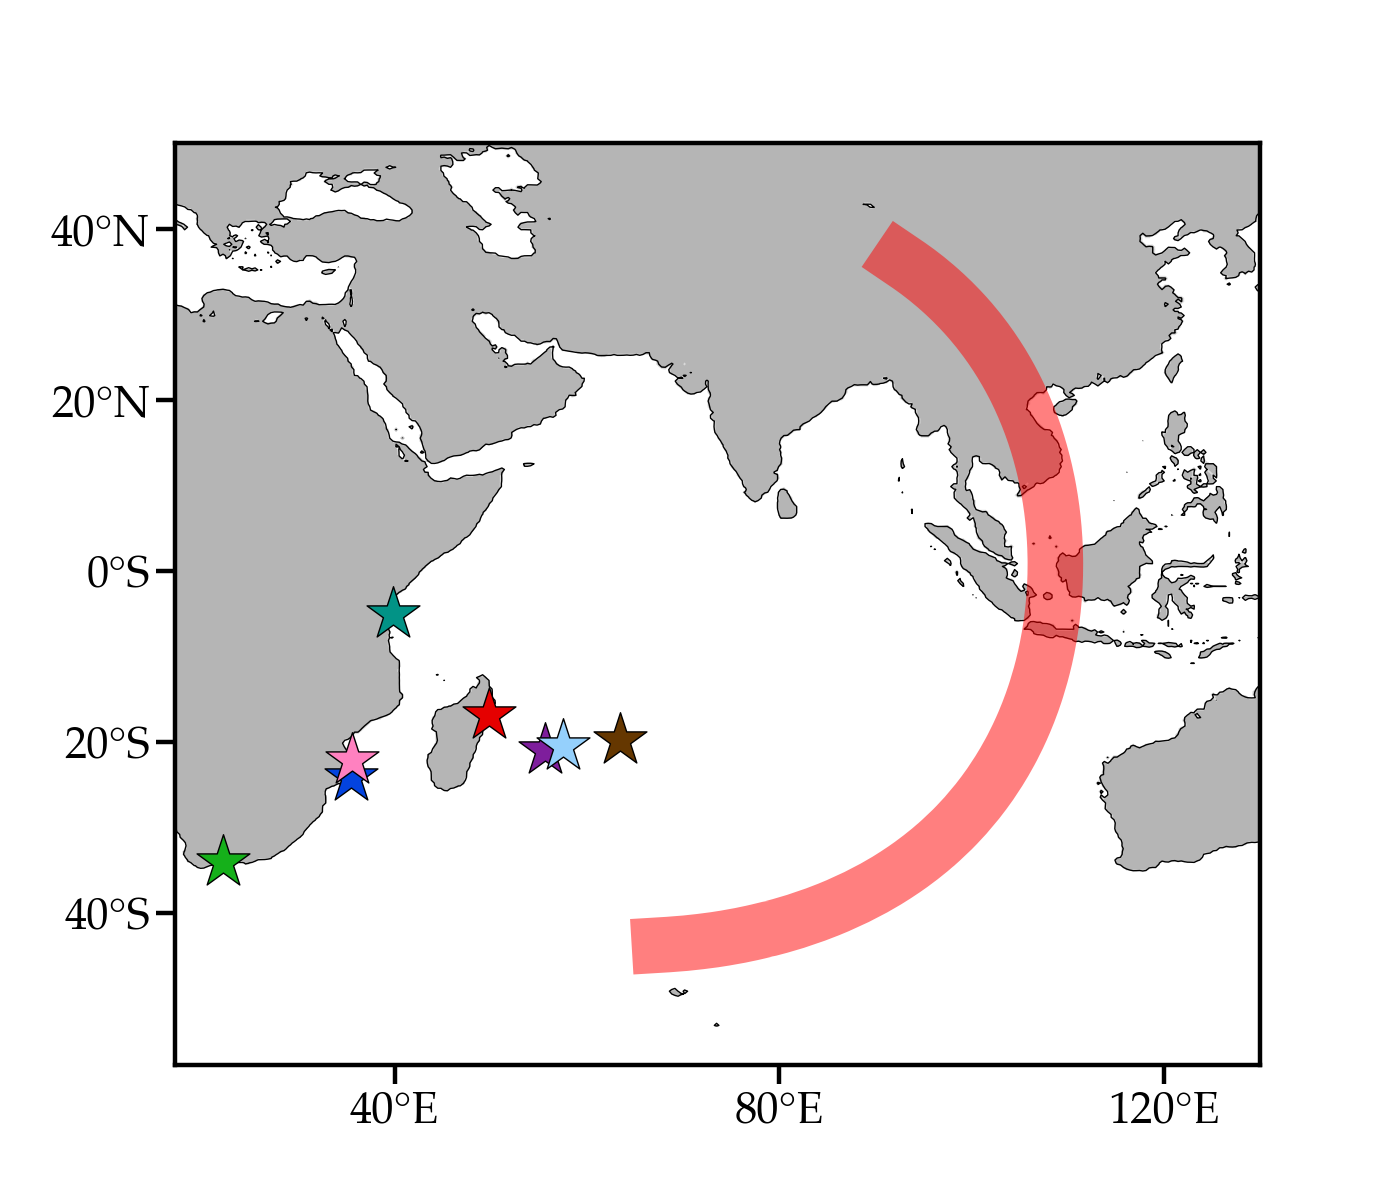
\includegraphics[width=0.85\textwidth]{figures/debris_map.png}
\end{figure}

\end{frame}

\section{Goal}
\begin{frame}{Goal}  

Using undrogued drifters,  which are subject to similar dynamics as floating debris, build a model to estimate the probable crash site.
\newline\newline
Model will utilize all available information:
\begin{itemize}
	\item last known satellite arc 
	\item debris beaching time and location
\end{itemize} 
\end{frame}

\section{Methodology}
\begin{frame}{Undrogued drifter trajectories since 1979}  

\begin{figure}[hbt]
  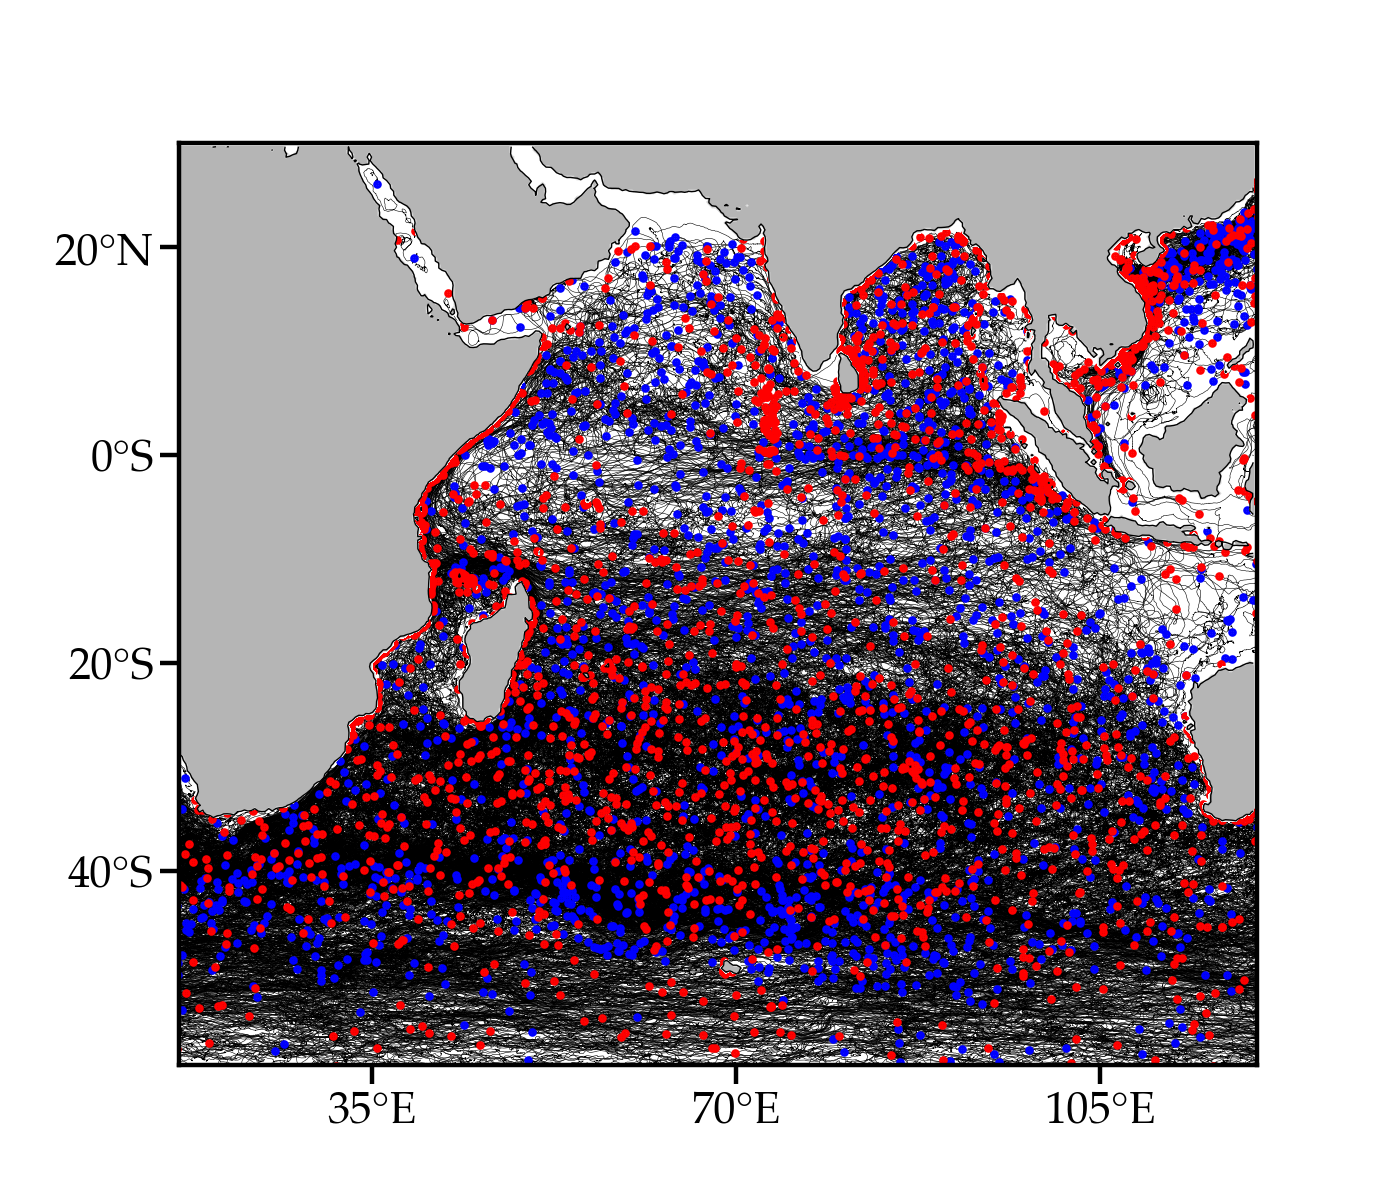
\includegraphics[width=0.85\textwidth]{figures/ioce-trajectories.png}
\end{figure}

\end{frame}

\begin{frame}{Average density of 226 drifters per bin}
\begin{figure}[hbt]
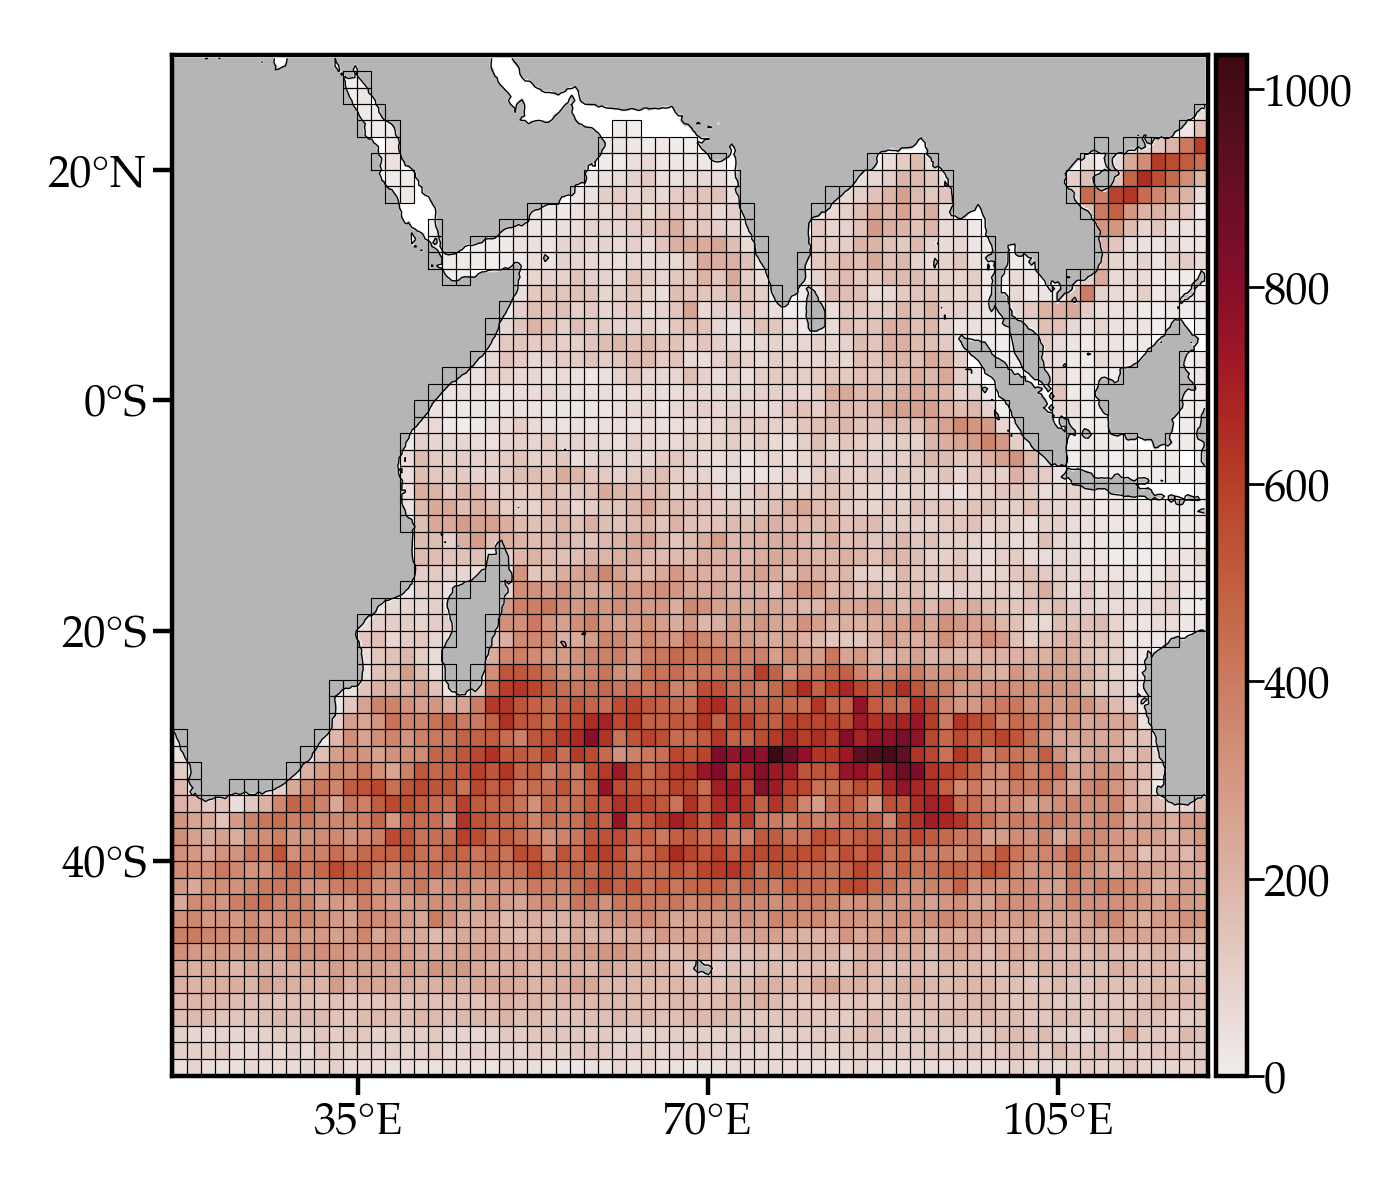
\includegraphics[width=0.85\textwidth]{figures/density.png}

\end{figure}
\end{frame}

\begin{frame}{Modelisation}

\begin{itemize}
  \item transition time: $T = 5$ days
  \item resolution: 2.5$^{\circ}$ $\times$ 2.5$^{\circ}$
  \item seasonality : three transition matrices (summer, winter, spring--fall)
\end{itemize}

\end{frame}



\begin{frame}{Long-term behavior}

Long-term behavior can be observed from the spectral analysis of the autonomous season-aware matrix:
\begin{equation*}
  P = P_\mathrm{W}^{18} \cdot P_\mathrm{SF}^{18} \cdot P_\mathrm{S}^{18}\cdot P_\mathrm{SF}^{18}
\end{equation*}
Note: $18 \cdot T = 90$ days $\approx$ 3 months.

\end{frame}

\begin{frame}{Quasistationnary distribution}
First approximation of the search area is obtain from the eigenvectors of the combined seasonal P along the satellite arc between the cyan dashed contour ($\approx 3600$\,km).

\begin{figure}[hbt]
  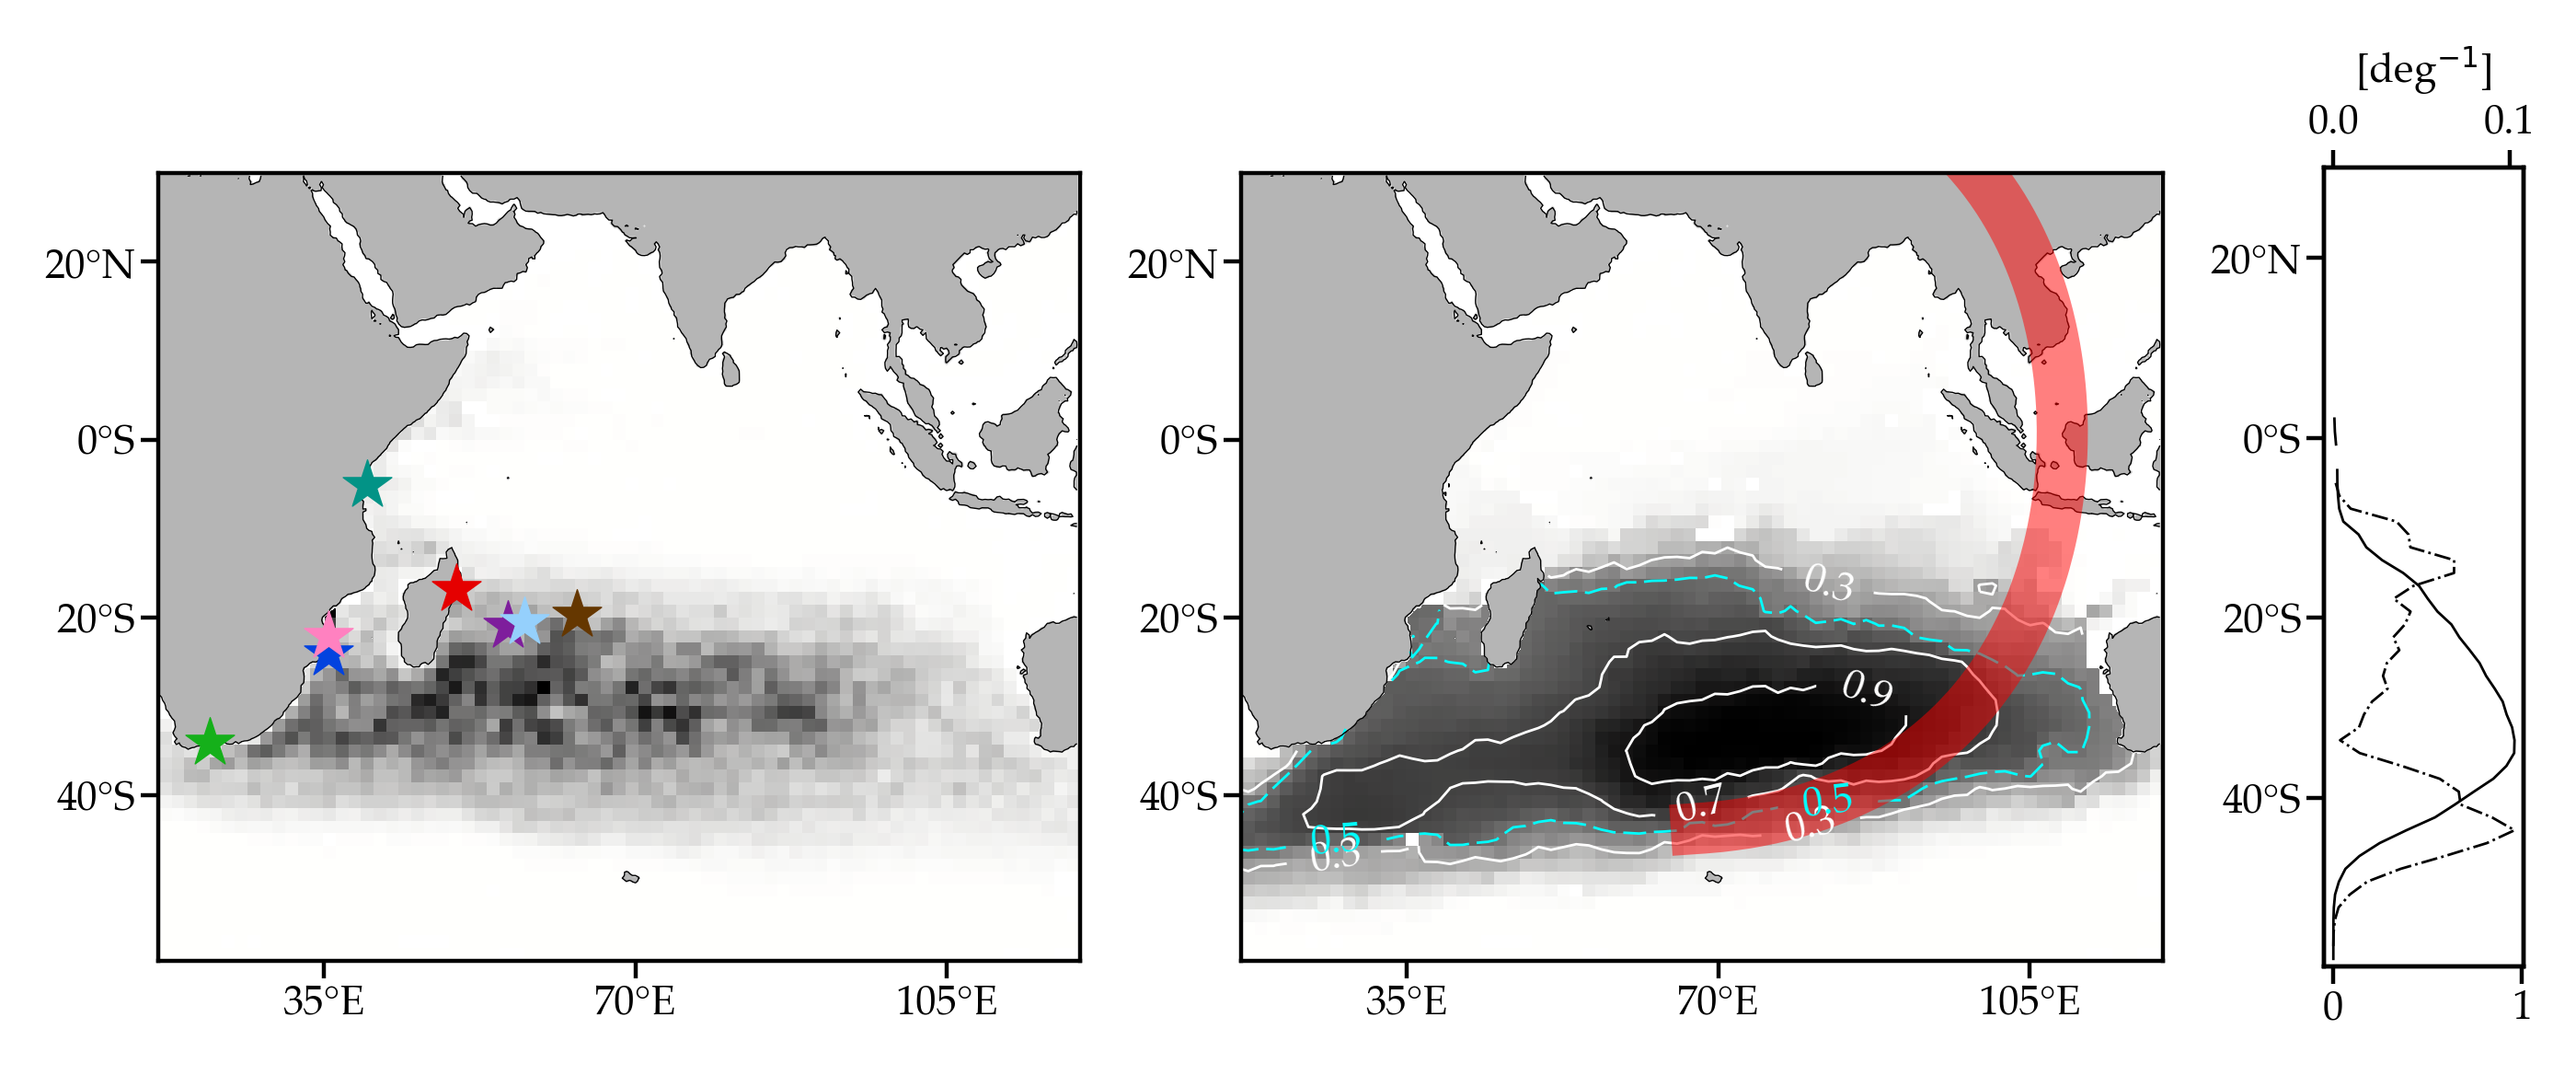
\includegraphics[width=\textwidth]{figures/mh370-fig02.png}
\end{figure}

\end{frame}

\begin{frame}{Bayesian Analysis}  
The Bayesian analysis uses the beaching events as observations to infer the probability distribution of the crash site.

\begin{itemize}
  \item Monsoon $P(t)$
  \item Mass exiting the domain terminates in a \textit{nirvana} state
  \item Beaching probability equals to the land ratio
\end{itemize}

\end{frame}

\begin{frame}{Probability to beach at the same time of the debris}
  \begin{equation}
  \tau^b := \inf_{k\ge 0}\{t+kT : \xi_{t+kT} = b\in \mathfrak B\}.
\end{equation}
Define $\Pr_c[\cdot] :=  \Pr[\,\cdot \mid \xi_t = c\in \mathfrak C]$ and
\begin{equation}
  p_c^b(k) := \mathbf 1_c P^k \cdot \mathbf 1_b,\quad c\in
  \mathfrak C,\, b\in \mathfrak B,
\end{equation}
where $\mathbf 1_j = (\delta_{ij})_{i\in S \cup
\{N+1\} \cup \mathfrak B}$, and then note that
\begin{equation}
  \Pr_c[\tau^b = t+kT] = 
  \begin{cases} 
   p_c^b(k) = 0           & \text{if } k = 0,\\
   p_c^b(k) - p_c^b(k-1)  & \text{if } k > 0.
  \end{cases}
  \label{eq:p}
\end{equation}
\end{frame}

\begin{frame}{Heatmap}

\begin{figure}[hbt]
  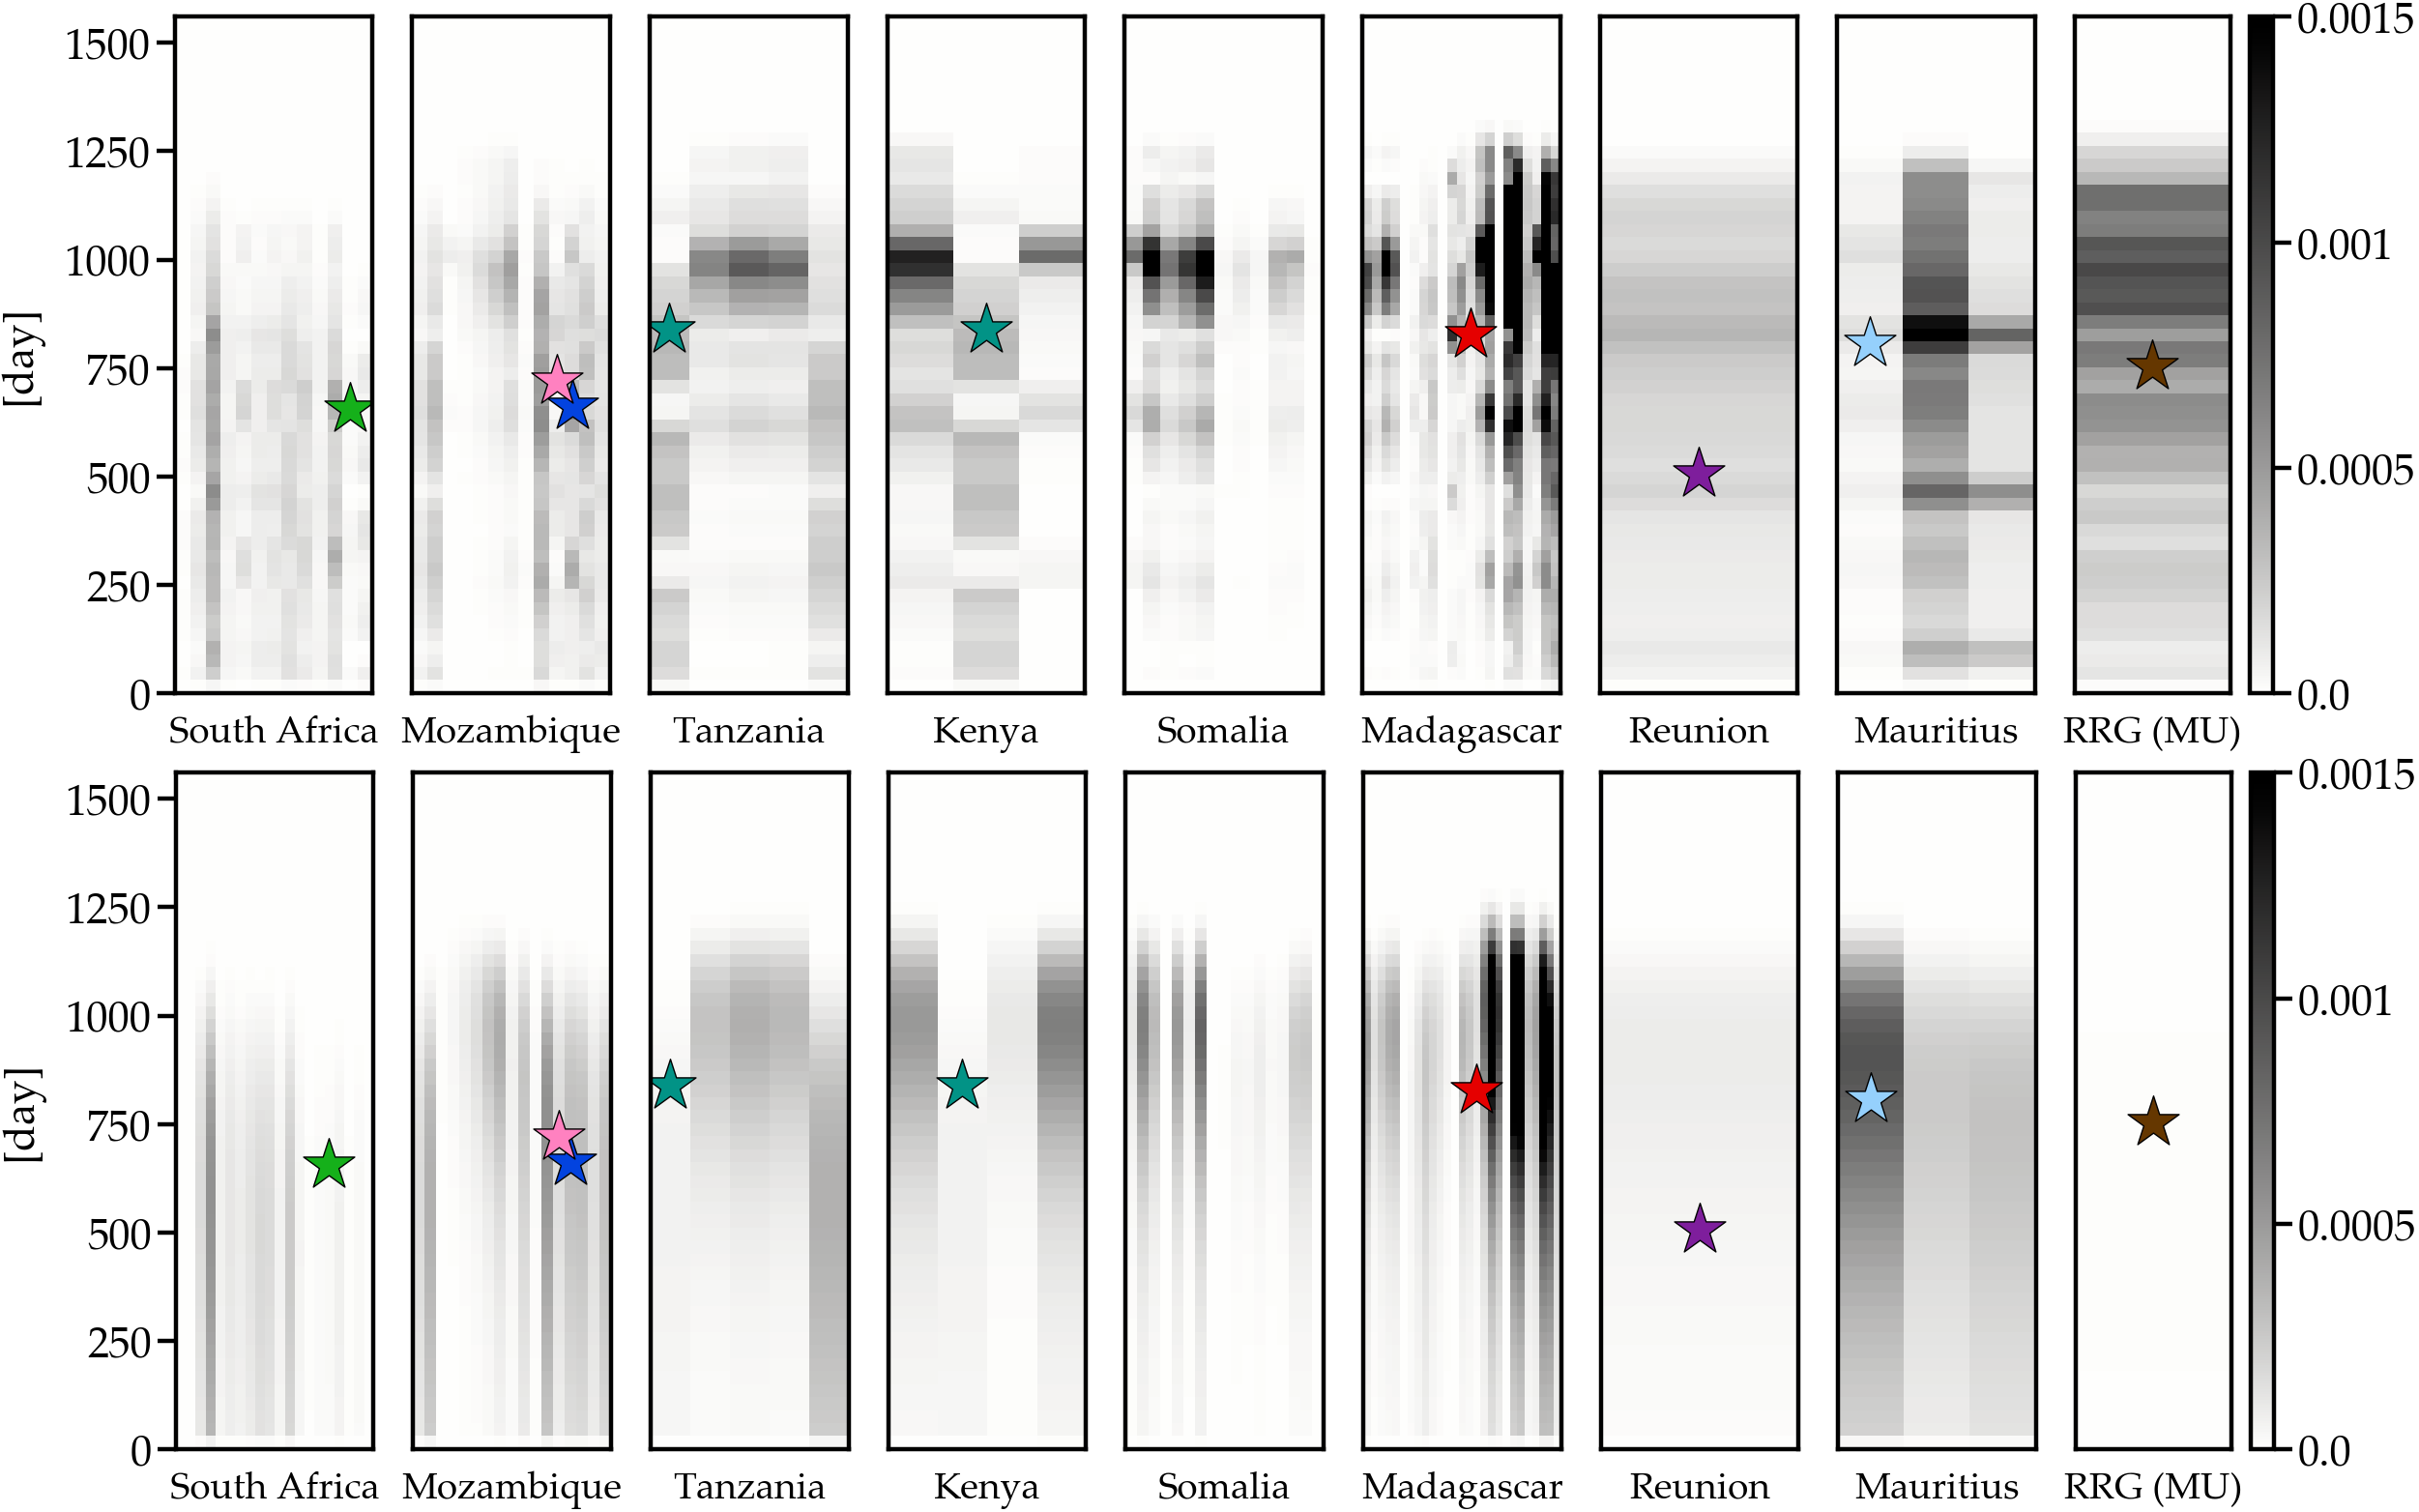
\includegraphics[width=\textwidth]{figures/mh370-fig03-si.png}
\end{figure}

\end{frame}


\begin{frame}

\begin{equation}
  p(t^\mathbf{b}|c) := \prod_{b\in \mathfrak B} p(t^b|c). 
\end{equation}

\end{frame}


\section{Results}

\begin{frame}{Bayesian Analysis}  

\begin{figure}[hbt]
  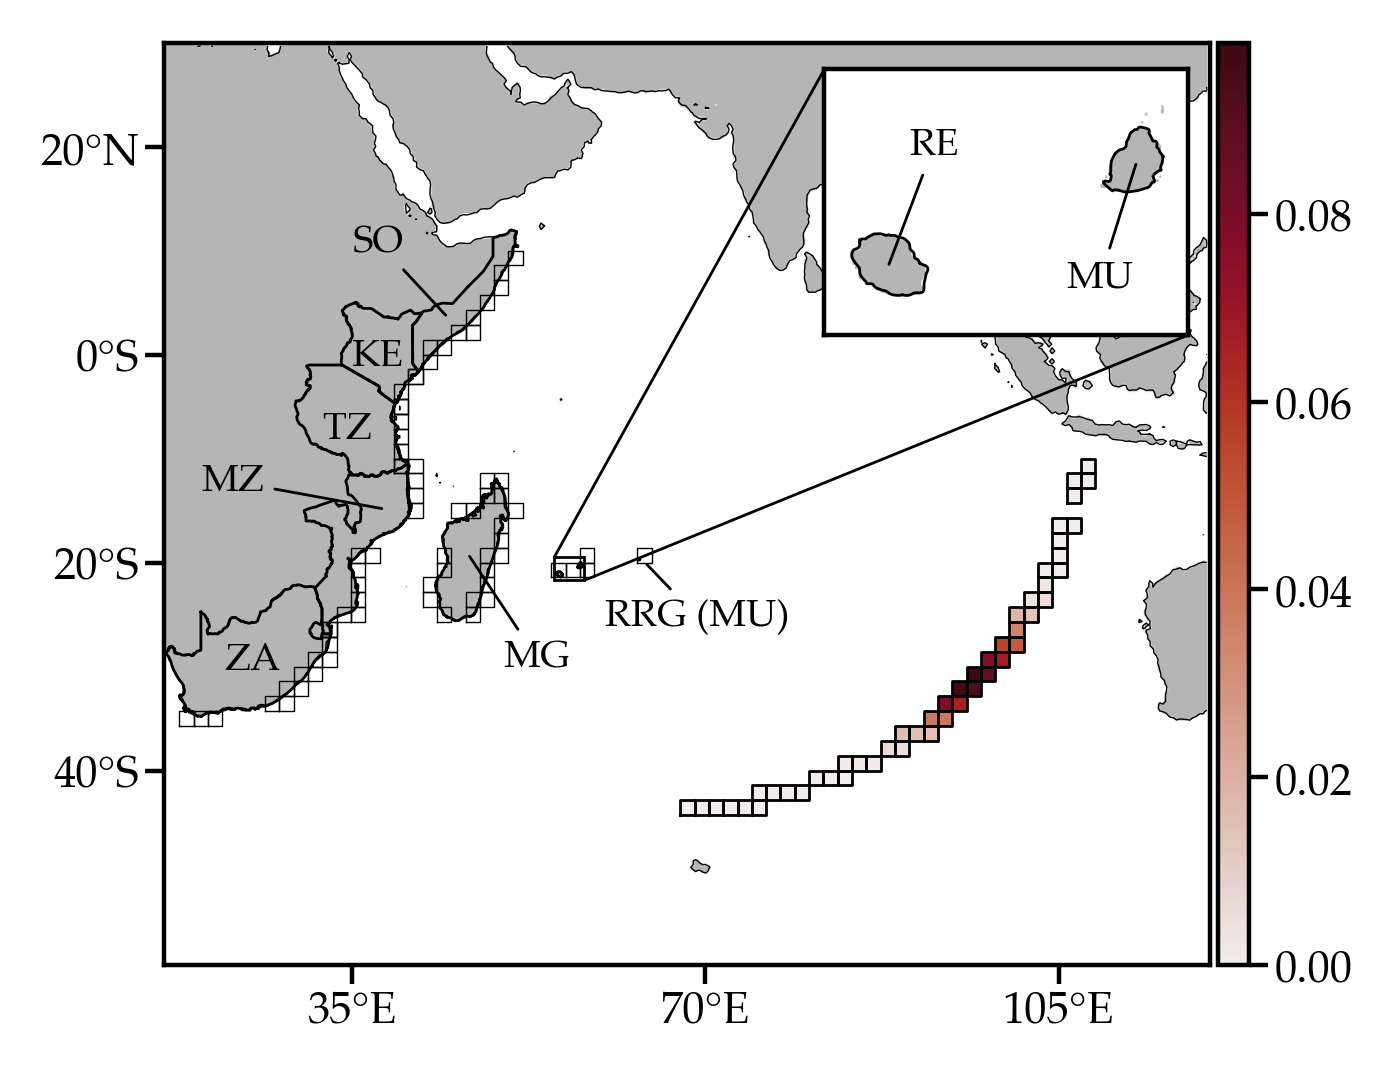
\includegraphics[width=0.85\textwidth]{figures/mh370-fig03.png}
\end{figure}

\end{frame}

\begin{frame}{Probability for each debris}  

\begin{figure}[hbt]
  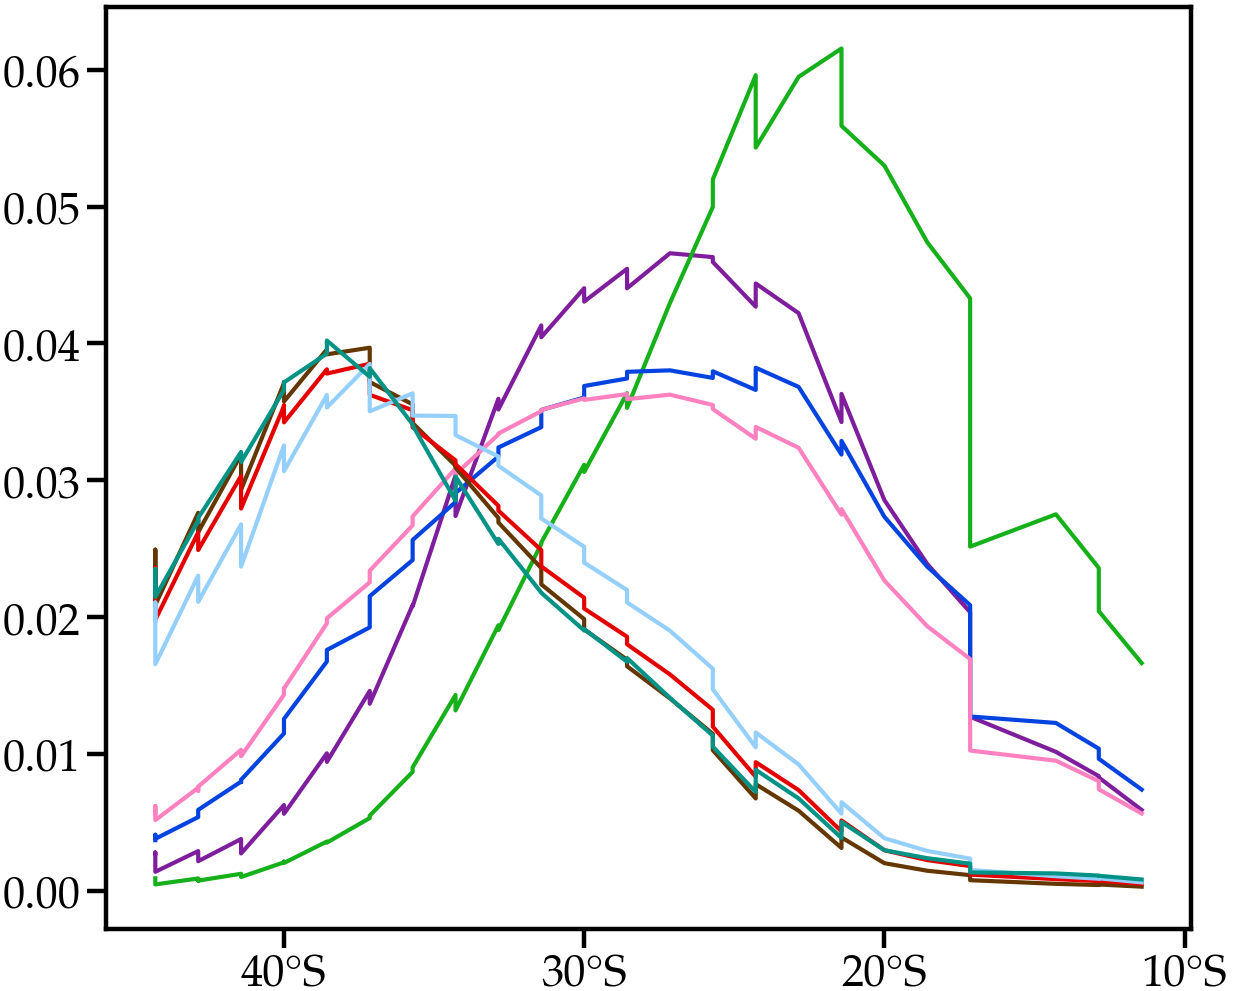
\includegraphics[width=0.8\textwidth]{figures/mh370-fig04.png}
\end{figure}

\end{frame}

\begin{frame}{Most probable paths}  

Explanation of the algorithm in simple words
\end{frame}

\begin{frame}{Most probable paths}  

\begin{figure}[hbt]
  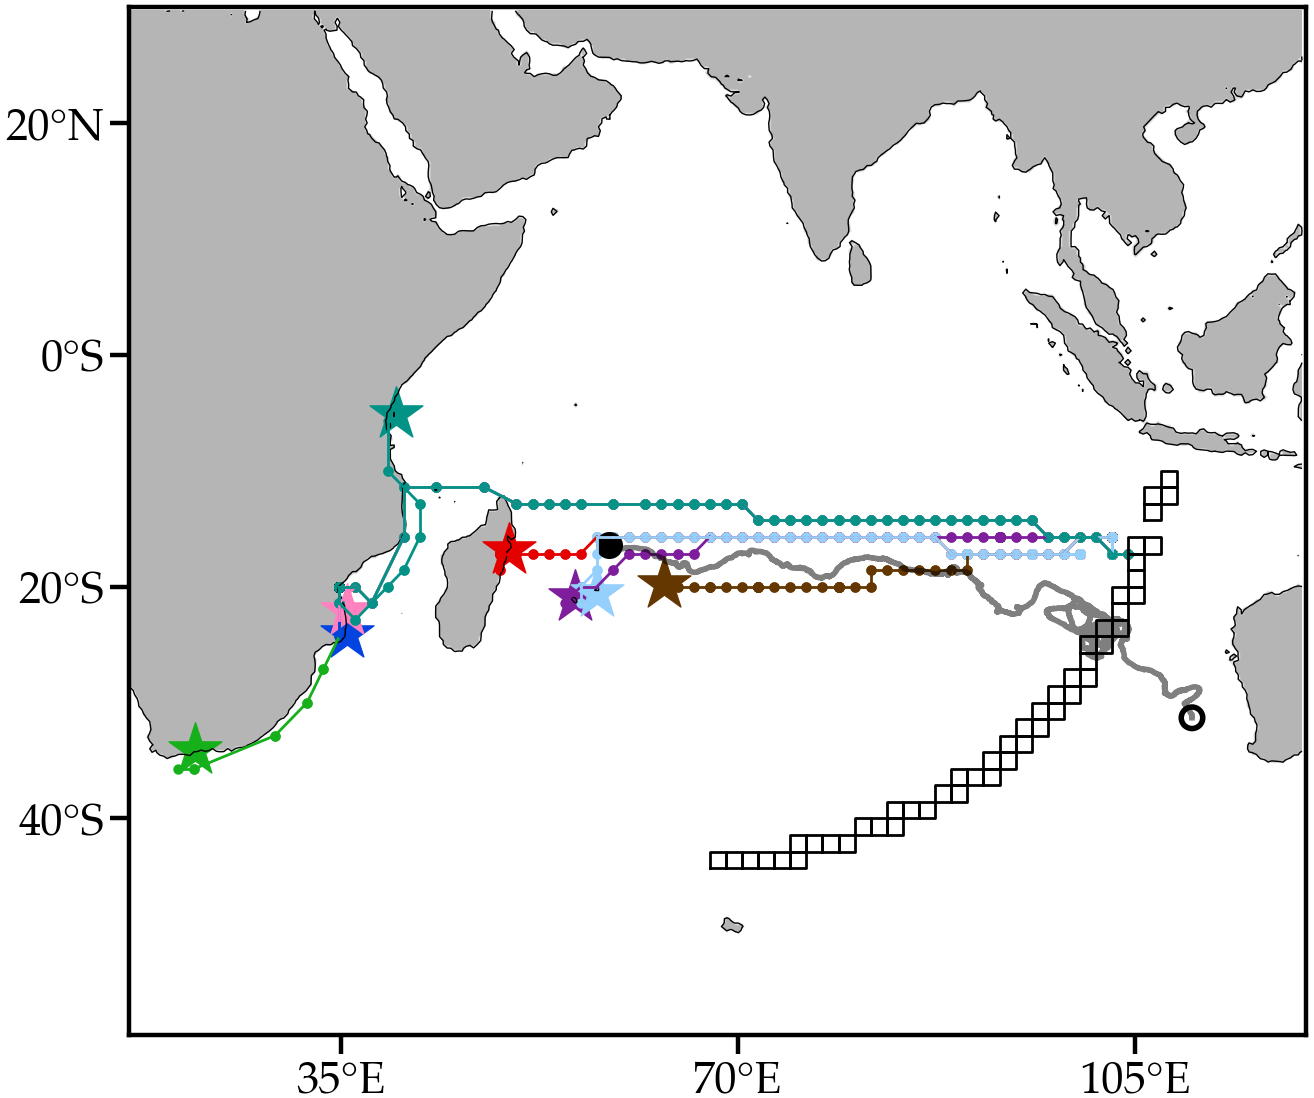
\includegraphics[width=0.85\textwidth]{figures/mh370-fig05.png}
\end{figure}

\end{frame}

\section{Conclusion}
\begin{frame}{Conclusion}

\begin{itemize}
	\item most likely position (next to second group)
	\item talk about news article that says it's probably north of the search site
	\item recirculation of first group cause delay
\end{itemize}
\end{frame}

\begin{frame}{References}
\printbibliography
\end{frame}

\end{document}